    %% BioMed_Central_Tex_Template_v1.06
%%                                      %
%  bmc_article.tex            ver: 1.06 %
%                                       %

%%IMPORTANT: do not delete the first line of this template
%%It must be present to enable the BMC Submission system to
%%recognise this template!!

%%%%%%%%%%%%%%%%%%%%%%%%%%%%%%%%%%%%%%%%%
%%                                     %%
%%  LaTeX template for BioMed Central  %%
%%     journal article submissions     %%
%%                                     %%
%%          <8 June 2012>              %%
%%                                     %%
%%                                     %%
%%%%%%%%%%%%%%%%%%%%%%%%%%%%%%%%%%%%%%%%%


%%%%%%%%%%%%%%%%%%%%%%%%%%%%%%%%%%%%%%%%%%%%%%%%%%%%%%%%%%%%%%%%%%%%%
%%                                                                 %%
%% For instructions on how to fill out this Tex template           %%
%% document please refer to Readme.html and the instructions for   %%
%% authors page on the biomed central website                      %%
%% http://www.biomedcentral.com/info/authors/                      %%
%%                                                                 %%
%% Please do not use \input{...} to include other tex files.       %%
%% Submit your LaTeX manuscript as one .tex document.              %%
%%                                                                 %%
%% All additional figures and files should be attached             %%
%% separately and not embedded in the \TeX\ document itself.       %%
%%                                                                 %%
%% BioMed Central currently use the MikTex distribution of         %%
%% TeX for Windows) of TeX and LaTeX.  This is available from      %%
%% http://www.miktex.org                                           %%
%%                                                                 %%
%%%%%%%%%%%%%%%%%%%%%%%%%%%%%%%%%%%%%%%%%%%%%%%%%%%%%%%%%%%%%%%%%%%%%

%%% additional documentclass options:
%  [doublespacing]
%  [linenumbers]   - put the line numbers on margins

%%% loading packages, author definitions

%\documentclass[twocolumn]{bmcart}% uncomment this for twocolumn layout and comment line below
\documentclass{bmcart}

%%% Load packages
%\usepackage{amsthm,amsmath}
%\RequirePackage{natbib}
%\RequirePackage[authoryear]{natbib}% uncomment this for author-year bibliography
\RequirePackage{hyperref}
\usepackage[utf8]{inputenc} %unicode support
%\usepackage[applemac]{inputenc} %applemac support if unicode package fails
%\usepackage[latin1]{inputenc} %UNIX support if unicode package fails
\usepackage{graphicx}

\usepackage[noabbrev]{cleveref}
\usepackage{siunitx}
\DeclareSIUnit \basepair{bp}
\DeclareSIUnit \byte{B}
\DeclareSIPrefix\mebi{Mi}{10}
\DeclareSIPrefix\gibi{Gi}{10}

\usepackage{biocon}
\newplant{At}{genus=Arabidopsis,epithet=thaliana}

%%%%%%%%%%%%%%%%%%%%%%%%%%%%%%%%%%%%%%%%%%%%%%%%%
%%                                             %%
%%  If you wish to display your graphics for   %%
%%  your own use using includegraphic or       %%
%%  includegraphics, then comment out the      %%
%%  following two lines of code.               %%
%%  NB: These line *must* be included when     %%
%%  submitting to BMC.                         %%
%%  All figure files must be submitted as      %%
%%  separate graphics through the BMC          %%
%%  submission process, not included in the    %%
%%  submitted article.                         %%
%%                                             %%
%%%%%%%%%%%%%%%%%%%%%%%%%%%%%%%%%%%%%%%%%%%%%%%%%


%\def\includegraphic{}
%\def\includegraphics{}

\usepackage{todonotes}
\setlength{\marginparwidth}{3cm}

\newcounter{todocounter}
\newcommand{\ff}[1]
{\stepcounter{todocounter}
 \todo[color=blue!40,author=For Frank]{\thetodocounter: #1}
 }
\newcommand{\ak}[1]
{\stepcounter{todocounter}
 \todo[color=green!40,author=Arthur]{\thetodocounter: #1}
 }


%%% Put your definitions there:
\startlocaldefs
\newcommand{\formatprogramnames}[1]{\texttt{#1}}
\newcommand{\ce}{\formatprogramnames{chloroExtractor}}
\newcommand{\oa}{\formatprogramnames{ORG.Asm}}
\newcommand{\fp}{\formatprogramnames{Fast-Plast}}
\newcommand{\ioga}{\formatprogramnames{IOGA}}
\newcommand{\np}{\formatprogramnames{NOVOPlasty}}
\newcommand{\go}{\formatprogramnames{GetOrganelle}}
\newcommand{\cassp}{\formatprogramnames{Chloroplast assembly protocol}}

\newcommand{\zenododataset}{\cite{zenododataset}}
\newcommand{\zenodorepo}{\cite{zenodorepo}}

\newcommand{\genename}[1]{\textit{#1}}

% Niklas table
%\newcommand{\ok}{\textcolor[rgb]{0.7,0.7,0}{\textsc{\bfseries{}OKAY}}}
%\newcommand{\bad}{\textcolor{red}{\textsc{\bfseries{}BAD}}}
%\newcommand{\good}{\textcolor[rgb]{0,0.6,0}{\textsc{\bfseries{}GOOD}}}
\newcommand{\ok}{\textsc{Okay}}
\newcommand{\bad}{\textsc{Bad}}
\newcommand{\good}{\textsc{Good}}


% List of docker images
\newcommand{\docker}[2]{\href{https://cloud.docker.com/u/chloroextractorteam/repository/docker/chloroextractorteam/#1}{chloroextracteam/#1:#2}}
\newcommand{\dockerce}{\docker{benchmark\_chloroextractor}{v2.0.0}}
\newcommand{\dockercesha}{\texttt{8f49e03424b37e699c5fea9391f79dbb9f2d0dc550ce86c4c700f39deec2dacd}}
\newcommand{\dockeroa}{\docker{benchmark\_org-asm}{v2.0.0}}
\newcommand{\dockeroasha}{\texttt{ff83677c97b7c4e346191b9e04a5162eeea2a8dfd9e60ff84067d33747868f60}}
\newcommand{\dockerfp}{\docker{benchmark\_fastplast}{v2.0.0}}
\newcommand{\dockerfpsha}{\texttt{a3d06a610f8340ba49c3ff3b27342534e2a5348b17caa4fd3c3f3d327243a272}}
\newcommand{\dockerioga}{\docker{benchmark\_ioga}{v2.0.0}}
\newcommand{\dockeriogasha}{\texttt{4698a21c343c60290bbf16811165a654ff01e8fddeb41cd75d0771b7f45968c0}}
\newcommand{\dockernp}{\docker{benchmark\_novoplasty}{v2.0.0}}
\newcommand{\dockernpsha}{\texttt{106387bad4e8e5c53fb9d4c3bdd60cdddf05a47b52a38697369eeabb947c547c}}
\newcommand{\dockergo}{\docker{benchmark\_getorganelle}{v2.0.0}}
\newcommand{\dockergosha}{\texttt{2ed3a464a82025a196ea56c649d0b0a3472cef76994bb065d56054d93298d956}}
\newcommand{\dockercassp}{\docker{benchmark\_chloroplast\_assembly\_protocol}{v2.0.0}}
\newcommand{\dockercasspsha}{\texttt{d10d2317103d91fadec4cb1d5466ac109f23176ad74b6f44f0179175f050155d}}
\endlocaldefs


%%% Begin ...
\begin{document}

%%% Start of article front matter
\begin{frontmatter}

\begin{fmbox}
\dochead{Research}

%%%%%%%%%%%%%%%%%%%%%%%%%%%%%%%%%%%%%%%%%%%%%%
%%                                          %%
%% Enter the title of your article here     %%
%%                                          %%
%%%%%%%%%%%%%%%%%%%%%%%%%%%%%%%%%%%%%%%%%%%%%%

\title{The landscape of chloroplast genome assembly tools}

%%%%%%%%%%%%%%%%%%%%%%%%%%%%%%%%%%%%%%%%%%%%%%
%%                                          %%
%% Enter the authors here                   %%
%%                                          %%
%% Specify information, if available,       %%
%% in the form:                             %%
%%   <key>={<id1>,<id2>}                    %%
%%   <key>=                                 %%
%% Comment or delete the keys which are     %%
%% not used. Repeat \author command as much %%
%% as required.                             %%
%%                                          %%
%%%%%%%%%%%%%%%%%%%%%%%%%%%%%%%%%%%%%%%%%%%%%%

\author[
    addressref={aff1,aff3},
    noteref={n1},
    email={jan.freudenthal@uni-wuerzburg.de}
    ]{\inits{JAF}\fnm{Jan A} \snm{Freudenthal}}
\author[
    addressref={aff1,aff2},
    noteref={n1},
    email={simon-pfaff@gmx.de}
    ]{\inits{SP}\fnm{Simon} \snm{Pfaff}}
\author[
   addressref={aff1,aff3},
   email={niklas.terhoeven@uni-wuerzubrg.de}
]{\inits{NT}\fnm{Niklas} \snm{Terhoeven}}
\author[
   addressref={aff1},
   email={arthur.korte@uni-wuerzubrg.de}
]{\inits{AK}\fnm{Arthur} \snm{Korte}}
\author[
   addressref={aff1,aff3,aff2 },
   noteref={n2},
   email={markus.ankenbrand@uni-wuerzubrg.de}
]{\inits{MJA}\fnm{Markus J} \snm{Ankenbrand}}
\author[
   addressref={aff2,aff4},                   % id's of addresses, e.g. {aff1,aff2}
   corref={aff1},                       % id of corresponding address, if any
   noteref={n2},                        % id's of article notes, if any
   email={frank.foerster@uni-wuerzburg.de}   % email address
]{\inits{FF}\fnm{Frank} \snm{Förster}}


%%%%%%%%%%%%%%%%%%%%%%%%%%%%%%%%%%%%%%%%%%%%%%
%%                                          %%
%% Enter the authors' addresses here        %%
%%                                          %%
%% Repeat \address commands as much as      %%
%% required.                                %%
%%                                          %%
%%%%%%%%%%%%%%%%%%%%%%%%%%%%%%%%%%%%%%%%%%%%%%


\address[id=aff1]{%
  \orgname{Center for Computational and Theoretical Biology, University of W\"{u}rzburg},
  \street{Campus Hubland Nord},
  \postcode{97074}
  \city{W\"{u}rzburg},
  \cny{Germany}
}

\address[id=aff3]{%
  \orgname{AnaLife Data Science},
  \street{Friedrich-Bergius-Ring 15},
  \postcode{97076}
  \city{W\"{u}rzburg},
  \cny{Germany}
}
\address[id=aff2]{%                           % unique id
  \orgname{Department of Bioinformatics, University of W\"{u}rzburg}, % university, etc
  \street{Biozentrum, Am Hubland},                     %
  \postcode{97074},                                % post or zip code
  \city{W\"{u}rzburg},                              % city
  \cny{Germany}                                    % country
}

\address[id=aff4]{%
  \orgname{Fraunhofer IME-BR},
  \street{Winchester Str.\ 2},
  \postcode{97076}
  \city{Gie\ss{}en},
  \cny{Germany}
}

%%%%%%%%%%%%%%%%%%%%%%%%%%%%%%%%%%%%%%%%%%%%%%
%%                                          %%
%% Enter short notes here                   %%
%%                                          %%
%% Short notes will be after addresses      %%
%% on first page.                           %%
%%                                          %%
%%%%%%%%%%%%%%%%%%%%%%%%%%%%%%%%%%%%%%%%%%%%%%

\begin{artnotes}
%\note{Sample of title note}     % note to the article
\note[id=n1]{Equal contributor} % note, connected to author
\note[id=n2]{Corresponding author} % note, connected to author
\end{artnotes}

\end{fmbox}% comment this for two column layout

%%%%%%%%%%%%%%%%%%%%%%%%%%%%%%%%%%%%%%%%%%%%%%
%%                                          %%
%% The Abstract begins here                 %%
%%                                          %%
%% Please refer to the Instructions for     %%
%% authors on http://www.biomedcentral.com  %%
%% and include the section headings         %%
%% accordingly for your article type.       %%
%%                                          %%
%%%%%%%%%%%%%%%%%%%%%%%%%%%%%%%%%%%%%%%%%%%%%%
\begin{abstractbox}
\begin{abstract} % abstract
%One or two sentences providing a basic introduction to the field, comprehensible to a scientist in any discipline.
Chloroplasts are photosynthetic organelles in plant cells and contain their own genomic information.
That genome can be utilized in different scientific fields like phylogenetics or biotechnology.
%Two to three sentences of more detailed background, comprehensible to scientists in related disciplines.
Thus, different assemblers have been developed specialized in chloroplast assemblies.
Those assemblers often use the output of whole genome sequencing experiments as input.
Such sequencing data usually contain the complete chloroplast genome information, even if the sequencing aims for the core genome.
%One sentence clearly stating the general problem being addressed by this particular study.
Different assembly tools have never been systematically compared. %to each other concerning success rate or computational requirements.
%One sentence summarising the main result (with the words “here we show” or their equivalent).
Here we present a benchmark of seven chloroplast assembly tools, capable to succeed in more than \SI{60}{\percent} of real data sets.
%Two or three sentences explaining what the main result reveals in direct comparison to what was thought to be the case previously, or how the main result adds to previous knowledge.
Our results show significant differences between the tested assemblers in terms of generating whole chloroplast genome sequences and computational requirements.
Moreover, we suggest further development to improve user experience and success rate.
%One or two sentences to put the results into a more general context. 
In terms of reproducibility, we created docker images for each tested tool, which are available for the scientific community.
Following the presented guidelines, users are able to analyse and screen data sets for chloroplast genomes using only standard computer infrastructure.
%Two or three sentences to provide a broader perspective, readily comprehensible to a scientist in any discipline, may be included in the first paragraph if the editor considers that the accessibility of the paper is significantly enhanced by their inclusion. 
Thus large scale screening for chloroplasts as hidden treasures within genomic sequencing data is feasible.

%\ff{Abstract}
%Useful as always: \url{https://cbs.umn.edu/sites/cbs.umn.edu/files/public/downloads/Annotated_Nature_abstract.pdf}
%The special issue will accept manuscripts presenting:
%
%- in-depth analyses of advantages
%
%-limitations of state-of-the-art methods
%
%-demonstration on a variety of representative datasets and simulations
%
%-clear guidelines/recommendations for the end-user
%
%-insight into future directions for methods
%\parttitle{First part title} %if any
%Text for this section.
%
%\parttitle{Second part title} %if any
%Text for this section.
\end{abstract}

%%%%%%%%%%%%%%%%%%%%%%%%%%%%%%%%%%%%%%%%%%%%%%
%%                                          %%
%% The keywords begin here                  %%
%%                                          %%
%% Put each keyword in separate \kwd{}.     %%
%%                                          %%
%%%%%%%%%%%%%%%%%%%%%%%%%%%%%%%%%%%%%%%%%%%%%%

\begin{keyword}
\kwd{Chloroplast}
\kwd{Genome}
\kwd{Assembly}
\kwd{Software}
\kwd{Benchmark}
\end{keyword}

% MSC classifications codes, if any
%\begin{keyword}[class=AMS]
%\kwd[Primary ]{}
%\kwd{}
%\kwd[; secondary ]{}
%\end{keyword}

\end{abstractbox}
%
%\end{fmbox}% uncomment this for twcolumn layout

\end{frontmatter}

%%%%%%%%%%%%%%%%%%%%%%%%%%%%%%%%%%%%%%%%%%%%%%
%%                                          %%
%% The Main Body begins here                %%
%%                                          %%
%% Please refer to the instructions for     %%
%% authors on:                              %%
%% http://www.biomedcentral.com/info/authors%%
%% and include the section headings         %%
%% accordingly for your article type.       %%
%%                                          %%
%% See the Results and Discussion section   %%
%% for details on how to create sub-sections%%
%%                                          %%
%% use \cite{...} to cite references        %%
%%  \cite{koon} and                         %%
%%  \cite{oreg,khar,zvai,xjon,schn,pond}    %%
%%  \nocite{smith,marg,hunn,advi,koha,mouse}%%
%%                                          %%
%%%%%%%%%%%%%%%%%%%%%%%%%%%%%%%%%%%%%%%%%%%%%%

%%%%%%%%%%%%%%%%%%%%%%%%% start of article main body
% <put your article body there>

%%%%%%%%%%%%%%%%
%% Background %%
%%
\section*{Introduction}
\subsection*{General introduction and motivation}
Chloroplasts are essential organelles present in plant cells and the cells of some protists.
Chloroplasts enable the conversion of light energy into chemical energy via photosynthesis.
They harbor their own ribosomes and a circular DNA genome usually with a size between \SIrange{120}{160}{\kilo\basepair} \cite{palmer_1985}.
Because of this small size, the chloroplast genome has been an early target for sequencing.
The first chloroplast genome sequences were obtained as early as 1986 \cite{ohyama_chloroplast_1986,shinozaki_complete_1986}.
These early efforts elucidated the general genome organization and structure of the chloroplast DNA. 
Chloroplast genome content and structure are reviewed for example in \cite{wicke_evolution_2011,green_chloroplast_2011}.
Chloroplast genomes are widely used for evolutionary analyses \cite{martin_plastid_2010,xiao-ming_inferring_2017}, barcoding \cite{kress_use_2005,hollingsworth_dna_2009,de_vere_dna_2015}, and meta-barcoding \cite{bell_review_2016,deiner_environmental_2017}.
Interesting aspects of chloroplast genomes are their small size (\SIrange{120}{160}{\kilo\basepair},\cite{palmer_1985}), caused through endosymbiotic gene transfer \cite{martin_evolutionary_2002,timmis_endosymbiotic_2004} and the low number of \numrange{100}{120} genes that are still encoded on the chloroplast genome \cite{wicke_evolution_2011}.
Despite the overall high conservation of the genome sequence, there are striking differences in the gene content between different groups (e.g. the loss of the whole \genename{ndh} gene family in Droseraceae \cite{nevill_plastome-wide_2019}). Even more extreme evolutionary cases, where chloroplasts show a very low GC content and a modified genetic code are described \cite{su_novel_2019}.

These differences call for comparative genomic approaches.
Given the small size, it is much easier to decipher the complete chloroplast genome than the complete core genome.
For example the \plant{At} core genome is approximately \SI{125}{\mega\basepair} in length \cite{schmuths2004,cao2011} while the size of the \plant{At} chloroplast genome with \SI{154}{\kilo\basepair} is more than \SI{800}{\times} smaller \cite{sato1999}.

Even if only a single chloroplast is located inside a plant cell, several hundreds copies of the chloroplast genome exists in each cell \cite{kumar_2014,bendich_1987}.
Therefore, many genome sequencing projects contain chloroplast reads as by-product.
In some cases the chloroplast data is even considered contamination and experimental protocols for reducing their content have been developed \cite{lutz_isolation_2011}.
An alternative approach to improve the assembly of the core genome would be to first resolve the chloroplast genome and afterwards use this information to remove those reads that map to the chloroplast genome.

Structurally, two inverted repeats (IR\textsubscript{A} and IR\textsubscript{B}) of \SIrange{10}{76}{\kilo\basepair} divide the chloroplast genome into a large (LSC) and a small single copy (SSC) region \cite{palmer_1985}.
Those large inverted repeats complicate automated resolution with short read technologies\cite{Wang2018}.
Moreover, the existence of different chloroplasts within a single individual, and thus multiple different chloroplast genomes, have been described for different plants \cite{corriveau_1988,Chat2002,Scar2016}.
Although the origin and evolutionary importance of this phenomena ---called heteroplasmy--- are only poorly understood, the assembly of whole chloroplast genomes might be hindered.  

Databases exist containing short read data for species where no reference chloroplast sequence is publicly available, eg.\ the Sequence Read Archive at NCBI \cite{sra2010}.
The availability of whole chloroplast genomes would enable large scale comparative studies \cite{tonti-filippini_what_2017}.
Additionally, reconstructed full chloroplast genomes have been used as super-barcodes \cite{coissac_barcodes_2016}, for biotechnology applications and genetic engineering \cite{daniell_chloroplast_2016}.

\subsection*{Approaches to extracting chloroplasts from whole genome data}

Different strategies have been developed to assemble chloroplast genomes \cite{twyford_strategies_2017}.
In general, obtaining a chloroplast genome from WGS data requires two steps. First, the chloroplast reads have to be extracted from the mixed sequencing data. 
The second step is the assembly and resolution of the special circular structure including the inverted repeats.
The extraction of the reads can be achieved by mapping the reads to a reference chloroplast. \cite{Vinga2012}.
A different approach that does not perform alignments, relies on the higher coverage of chloroplast data in the whole genome sequencing data set\cite{Chan2013}.
Here, a $k$-mer analysis can be used to extract the most frequent reads.
An example for this is implemented in \ce{} \cite{j_ankenbrand_chloroextractor:_2018}. %\todo{ce ist hier der einzig explizit genannte Assembler, das wirkt wie bias :) entfernen? Nope... Steht klar ein Beispiel und wir haben nun mal den angesehen... Würde ich jetzt einmal so drin lassen. Alternativ nehmen wir noch einen dazu}
A third method combines both approaches by using a reference chloroplast as seed and simultaneously assembling the reads based on $k$-mers \cite{dierckxsens_novoplasty:_2017}.

%\ak{e.g. HomBlocks: A multiple-alignment construction pipeline for organelle phylogenomics based on locally collinear block searching, aber ist nicht inkluded, also können wir zitieren, müssen aber nicht}

\subsection*{Purpose and scope of this study}
The goal of this study is to compare the effectiveness and efficiency of existing open source command-line tools to de-novo assemble whole chloroplast genomes from raw genomic data sets with minimal configuration. 
This includes no need for extensive data preparation, no need for a specific reference (apart from \plant{At}), no need to change default parameters, no manual finishing.
We further restricted our benchmark to paired end Illumina data sets as these are routinely generated by modern sequencing platforms \cite{Goodwin2016}. 

In our opinion this reflects the most common use cases: (1) a user trying a tool quickly without digging into options for fine tuning and (2) large scale automatic applications.
Still, we acknowledge that the performance of the tools might be significantly improved by optimizing parameters (and references if applicable) for each data set specifically.
However, an exhaustive comparison - including tuning of all different possible parameters for each tool- was out of scope for this study. 

Our results will enable the discovery of novel chloroplast genomes as well as an assembly of inter/intra-individual differences in the respective chloroplast genomes.  

\section*{Methods}
\subsection*{Data availability}
Source code for all methods used is available at \cite{github-benchmark-repo} and archived in zenodo under \zenodorepo{}.
All docker images are published on \cite{dockerhub-benchmark} and are named with a leading \texttt{benchmark\_} (\cref{tab:dockerimages}).

To enable a fair comparison of all tools, we generated simulated sequencing data.
Those simulated data sets are stored at \zenododataset{}.
This study adheres to the guidelines for computational method benchmarking \cite{weber_essential_2018}.

\subsection*{Tool Selection}
We included tools designed for assembling chloroplasts from whole genome paired end Illumina sequencing data. As a requirement, all tools must be available as open source software and allow execution via a command line interface. 
As a graphical user interface is not suitable for automated comparisons, tools only providing a graphical interface have not been included.
The following tools were determined to be within the scope of this study:
\oa{} \cite{coissac_barcodes_2016}, 
\ce{} \cite{j_ankenbrand_chloroextractor:_2018}, 
\fp{} \cite{mckain__fast-plast_2017}, 
\ioga{} \cite{bakker_herbarium_2016}, 
\np{} \cite{dierckxsens_novoplasty:_2017}, 
\go{} \cite{jin_getorganelle:_2018}, and
\cassp{} \cite{sancho_comparative_2018}.

Other related tools for assembling chloroplasts that did not meet our criteria and are therefore outside the scope of this study are for example:
\texttt{Organelle PBA} \cite{Soorni2017}, \texttt{sestaton/Chloro} \cite{sestaton}, \texttt{Norgal}  \cite{Al-Nakeeb2017}, and \texttt{MitoBim} \cite{mitobim2013}.

\texttt{Organelle PBA} is designed for PacBio data and does not work with paired Illumina data alone.
\texttt{sestaton/Chloro} fits our criteria, but it is flagged as work in progress and development and support seem to have ended two years ago.
\texttt{Norgal} is a tool to extract organellar DNA from whole genome data based on a \textit{k}-mer frequency approach. However the final output is a set of contigs of mixed mitochondrial and plastid origin. The suggested approach to get a finished chloroplast genome is to run \np{} on the ten longest contigs. Therefore we only included \np{} with the default settings and excluded \texttt{Norgal}.
\texttt{MitoBim} is specifically designed for mitochondrial genomes. Even though there is a claim by the author that it can be used for chloroplasts as well, there is no further description on how to do that \cite{mitobim_issue16}.

Additionally, there is a protocol for the \texttt{Geneious} \cite{geneious} software available \cite{geneious-protocol}.
However, \texttt{Geneious} is closed source and GUI based, which is not in the scope of this study.
There is also another publication describing a method for assembling chloroplasts \cite{method-description-paper}.
However, the link to the software is not active anymore.

\subsection*{Our Setup}
We want to use a minimum of different parameter settings for all assembly programs to enable a fair comparison. 
Therefore, we decided to specify that all programs have to work based on two input files, representing a data set's forward (\texttt{forward.fq}) and reverse  (\texttt{reverse.fq}) sequence file in FASTQ format.
Depending on the assembler, output files with different names and locations are generated.
Those different files are copied and renamed to ensure that each assembly approach produces the same output file (\texttt{output.fa}). 
Additionally, we set an environment variable for all programs to control the number of allowed threads.
All three requirements (defined input file names, defined output file name, thread number control via environment variable) are ensured by a simple wrapper script (\texttt{wrapper.sh}).
Finally, for a maximum of reproducibility all programs have been bundled into individual docker images based on a central base image which provides all the required software. Those docker images were used for the recording of the consumption of computational resources.
Furthermore, all our docker images have been converted into singularity containers for the quantitative measurement on simulated and real data sets.
Singularity container were built from docker images for usage on a HPC-environment using Singularity v.2.5.2 \cite{kurtzer2017singularity}
All singularity containers were run on %the Julia-HPC 
Intel® Xeon® Gold \num{6140} Processors using a Slurm workload manager version 17.11.8 \cite{Jette02slurm}. Assemblies were run on \num{4} threads using \SI{10}{\gibi\byte} RAM with a time limit of \SI{48}{\hour}. 
\subsection*{Data}
\subsubsection*{Simulated}
To avoid suffering from sequencing errors and biological variances, we simulated perfect reads based on the \plant{At} (TAIR10) chloroplast assembly \cite{tair10}.
We used a sliding window approach with \texttt{seqkit} \cite{seqkit}. The exact commands are documented in \href{https://github.com/chloroExtractorTeam/benchmark/blob/master/03_representative_datasets.md}{\texttt{03\_representative\_datasets.md}} in \zenododataset{}.
For the final simulated data sets reads based on mixtures of the \plant{At} (TAIR10) core and chloroplast genome were generated with different ratios ( \num{0}:\num{1}, \num{1}:\num{10}, \num{1}:\num{100}, and \num{1}:\num{1000}).
Additionally, we generated data with different read lengths (\SIlist{150;250}{\basepair}). All data simulated contain exactly 2 million read pairs.

%(circular for chloro and mito). No errors, no insert size variation, perfect quality, equal coverage.

\subsubsection*{Real}
We selected real data deposited at SRA \cite{sra2010}.
We searched all data that matched  \texttt{((((((("green plants"[orgn]) AND "wgs"[Strategy]) AND "illumina"[Platform]) AND "biomol dna"[Properties]) AND "paired"[Layout]) AND "random"[Selection])) AND "public"[Access]} \cite{sra_search_term}. 
For each species with a reference chloroplast in CpBase \cite{cpbase}, we selected one data set of those.
In total, this accumulated to \num{369} data sets (see supplement for details).

\subsection*{Evaluation Criteria}
\subsubsection*{Computational Resources}
%Due to computational resources are limited, we evaluated the effect of different input parameters.
We recorded the mean and the peak CPU usage, the peak memory consumption, and the size of the assembly folder for each program. 
As input data, we used different data sets comprising \numlist{25000;250000;2500000} read pairs sampled from  our simulated reads.
%Therefore, the simulated perfect read files have been read repeatedly to achieve the required number of read pairs.
We used our docker image setup (\cref{tab:dockerimages}) to run all assembly programs three times for each parameter setting.
The different settings combined different input data and different number of threads to use (\numlist{1;2;4;8}).

Some programs will use more CPU threads than specified, therefore, the number of CPUs available have been fixed using the CPU option while running the docker run command.
For each assembly setting, we recorded the peak memory consumption, the CPU usage (mean and peak CPU usage) and the size of the folder where the assembly was calculated.
The values of CPU and memory usage have been obtained by docker.
The disk usage was estimated using the GNU tool \texttt{du}.
We used \texttt{GNU parallel} for queuing of the different settings \cite{Tange2011a}.

\subsubsection*{Qualitative}
The qualitative evaluation is mainly based on the reviewer guidelines for the Journal of Open Source Software (JOSS) \cite{joss}.
To create a standard environment, all tools were tested in a fresh default installation of Ubuntu 18.04.2 running in a virtual machine (VirtualBox Version 5.2.18\_Ubuntu r123745).
We chose this setup instead of the docker container, because it resembles a typical user environment better than the minimal docker installation.
The tools were installed according to their installation instructions and the provided tutorial or example usage was executed.
During the evaluation, the following questions were asked:

\begin{itemize}
    \item Is the tool easy to install? 
    \item Is there a way to test the installation or a tutorial on how to use the tool? 
    \item Is there a good documentation on the parameter settings? 
    \item Is the tool maintained (issues answered, implementation of new features)? 
    \item Is the tool Open Source?
\end{itemize}

These questions were answered with \good{}, \ok{} or \bad{}, depending on the quality of the result. 
For example, a \good{} installation utilizes an automated package or dependency management like \texttt{apt}, CRAN, docker, etc.
An \ok{} installation procedure provides a custom script to install everything or at least lists all dependencies.
A \bad{} installation procedure fails to list important dependencies or produces errors, that prevent a successful installation without exhaustive debugging.

After an initial evaluation, we contacted all authors via their GitHub or GitLab issue tracking to communicate potential flaws we found.

\subsubsection*{Quantitative}

%We use continuity: number of contigs.
%Completeness: Number of covered bases on reference (when aligning assembly).
%Correctness: Number of covered bases in assembly (when aligning reference).
%Repeat resolution: Difference between above two measures (indicates collapsed or expanded repeats)
%
%\nocite{oreg,schn,pond,smith,marg,hunn,advi,koha,mouse}


%We want to quantify continuity, completeness, correctness and repeat resolution.

For each data set and assembler the generated chloroplast genome was compared to the respective reference genome using a pairwise alignment obtained with \texttt{minimap2} v2.16 \cite{li2018minimap2}. Based on theses alignments a score is calculated as shown in \cref{eq:quantitative}
The assemblies were scored on a scale from 0 to 100, with 100 being the best and 0 the worst possible score. Four different metrics were Incorporated, each contributing  $\frac{1}{4}$ to the total score: Completeness, correctness, repeat resolution and continuity.
These metrics are similar in concept by those used in the Assemblathon 2 project: coverage, validity, multiplicity, and parsimony \cite{assemblathon2}.

The completeness is estimated as the coverage of the assembled chloroplast genome versus the reference genome ($cov_{ref}$)
It resembles how many bases of the query genome can be mapped to its respective reference genome.
Secondly, we mapped the reference genome against the query.
The coverage of the reference genome ($cov_{qry}$) is used as measurement for the correctness of the assembly.
The repeat resolution is estimated from the size difference of the assembly and the reference genome ($min\left\{ \frac{cov_{qry}}{cov_{ref}}, \frac{cov_{ref}}{cov_{qry}}\right\}$), leading to values between 0 and 1.
The fourth metric used is the continuity, represented by the number of contigs.
A perfect score is achieved if one circular chromosome was assembled, while the score gets worse with the amount of contigs.

\begin{equation}
   score = \frac{1}{4} \cdot \left( cov_{ref} +  cov_{qry} + min\left\{ \frac{cov_{qry}}{cov_{ref}}, \frac{cov_{ref}}{cov_{qry}}\right\} + \frac{1}{n_{contigs} }\right) \cdot 100 
   \label{eq:quantitative}
\end{equation}

\subsubsection*{Consistency}
To ensure consistency of the obtained results, we randomly chose  \num{100} data sets, that in the previous runs resulted in outputs for most of the assemblers and run them again with the same parameters as before.
The resulting assemblies were scored again as described and the scores of the first and the second run were compared to each other
This information is important to assess the robustness of the different programs.

\section*{Results}
\subsection*{Performance metrics}
%\subsection*{Computational Resources}
%Table and figure of performance evaluation. Including RAM, I/O, runtime, parallelization ability, CPU usage. Free text description of results, range, mean/median, effect of input size, threads parameter, ...

\subsubsection*{Time requirements}
In terms of run time, massive differences between the different tools have been observed. Apart from tool-specific differences, input data and number of threads had huge impact. The observed run times varied from a few minutes to several hours (\cref{fig:performance_runtime}).

Some assemblies failed to finish within the time-limit we set (\SI{48}{\hour}). 
On average the longest time to generate the assemblies was taken by \ioga{} and \fp{} followed by \oa{} and \go{} the most time efficient tool was \ce{}, which on average is a little faster than \np{} and \cassp{}.
%% multithreading

Not all the tools were able to benefit from having access to multiple threads. Both \np{} and \oa{} take about the same time independent of being able to utilize \numlist[list-final-separator={, or }]{1;2;4;8} threads. \cassp{}, \ce{}, \go  and \fp{} all profit from multi-threading (\cref{fig:performance_runtime}, \cref{fig:performance_memory_cpu}).

\subsubsection*{Memory and CPU Usage }
The peak and mean CPU usage, as well as peak memory and disk usage have been recorded for all assemblers based on the same input data set and number of threads to use (\cref{fig:performance_memory_cpu}).
Mainly, the size of the input data influenced the peak memory usage with the exception of \ce{} and \ioga{}.
Those two assemblers seems to have a memory usage pattern, which is less influenced by the size of the data.
The number of allowed threads had only a limited impact on the peak memory usage.
Nevertheless, all programs profit by a higher number of threads, if the size of the input data was increased.
In contrast, the disk usage is independent from input size and number of threads for all assemblers.
%but the factor between the programs exceeds a factor of \num{100}.

\subsection*{Qualitative}
The user experience of most tools was evaluated as mainly \good{} (\cref{tab:resultsQual}). However, a few critique points remained.
Two minor dependencies were missing in the \go{} installation instructions and there was no test data available.
Additionally, an issue occurred when running it on a \plant{At} data set.
We are currently in the process of resolving this with the authors.

The \fp{} installation instructions were missing some dependencies.
Like \go{}, \fp{} does not offer a test data set or a tutorial, except for some example commands. 

The \oa{} installation instructions did not work.
We found some issues, which are probably related to the requirement of \texttt{Python~3.7}.
There is a tutorial where sample data is available.
However, following the instructions resulted in a segmentation fault.
We found a workaround for this bug and contacted the authors.

The main critique point of \np{} was the lack of a test data set with instructions.
This was fixed by the authors after we contacted them.
Additionally, \np{} uses a custom license, where an OSI approved license would be preferred.

The \ce{} does come with a test data set and a short tutorial.
However, it is currently not possible to evaluate the results of the test run.

The \ioga{} installation instructions were missing many dependencies.
Also, there was no test data or tutorial available and there is no license assigned to it.
Since there was no update to the GitHub repository for the last three years, the project can be seen as inactive.
After contacting the authors, they promised to resolve the mentioned issues.

As many of the other tools, the installation instructions for the \cassp{} were missing some dependencies.
The list was updated after we contacted the authors.
This tool does come with a test data set, however a note about the expected outcome is missing.
A more extensive tutorial is provided.
The description about the parameter is short, but sufficient.

\subsection*{Quantitative}
\subsubsection*{Simulated data}
The only assembler obtaining perfect results according to our score for the simulated data sets is \go{} (\cref{fig:simulated}).
\ioga{} and \cassp{} showed the worst performance, being unable to fully assemble a single chloroplast out of \num{14} runs.
\np{} performed second best with scores above \num{80} for all data sets, only failing to resolve the contigs into one single circular chloroplast assembly.
The overall performance is best, when the input data consists purely of chloroplast reads.
Only \ioga{} and \cassp{} failed to deliver any results under this scenario once.
In general, no clear correlation between either length of the input reads or the ratio of core vs chloroplast reads and the performance of the different assemblers can be observed. 

\subsubsection*{Real data sets}
Concerning the performance of the assemblers on the real data sets, we were able to observe considerable differences in the median score (\cref{fig:swarmplot}).
The highest scores were achieved by \go{} with a median of \num{99.7} and \num{199} circular assemblies out of a total of 356 assemblies that resulted in an output (\cref{tab:scores}).
The performance of \go{} is followed by \fp{}, \np{}, \oa{}, and \ce{}. \fp{} is outperforming the latter two slightly in terms of score, with twice as much \num{114} perfectly assembled chloroplast genomes (\np{} produced \num{66} and \oa{} \num{55} circular genomes).
\ioga{} and \cassp{} were both not able to assemble a circular, single-contig genome (\cref{tab:scores}), consequently resulting in the lowest mean and median scores (\cref{fig:upset}).

%\textit{swarm plot goes here}
%% Den upset plot eventuell erst in die Discussion reinbringen ? Da wir davon ableiten welche tools wir empfehlen?

\subsubsection*{Consistency}
Consistency was tested by re-running assemblies and comparison of the scores of two assemblies (\cref{fig:consistency}).
Replicates that did not produce an output were manually scored as \num{0}. 
\go{} was the only tool that succeeded in obtaining similar scores for all assemblies, without producing and completely unsuccessful assemblies for this subset of data.
Except for \fp{} all the other tools had at least one assembly that was unsuccessful in one run, but produced an output in the other.
%\ak{oben steht \go{} war als einziges immer gut, dann kommt except for \fp{} ?? does not seem to be consistent}
Notably \ioga{} appears to have a tendency to perform differently in independent runs.
Here, more than \SI{10}{\percent} of the assemblies failed in one run only.

Both \fp{} and \np{} tend to have minor changes in the assembly when the overall performance is comparably well, leading to the arrow-shaped scatter plots.
%\ak{link to figure scatter plots is missing}
\ce{} and \cassp{} appear to be the most robust assemblers, having only few deviations between the two runs.

\section*{Discussion}
We aimed to generate an overall performance score for the different chloroplast assemblers, but depending on distinct downstream applications, the different criteria assessed in this work need to be weighted differently.
For example, ease of installation and use might not be a big concern if the tool is installed once and integrated in an automated pipeline. On the other hand this factor alone might prevent other users from being able to use the tool in the first place.
Similarly, computational requirements or run time might be less relevant, if the goal is to assemble a single chloroplast for further analysis, but it is essential if hundreds or thousands of samples should be processed in parallel for a large scale study.
Eventually, both ease of use and run time are irrelevant if the tool is not able to successfully accomplish its task.
Also the scope of this study needs to be considered when interpreting the guidelines below.
In particular, we evaluated all tools under the assumption that they are used in the most basic form (default parameters, no hand selected reference, no pre-processing of the data or post-processing of the result, restricted run time).
It is important to note that any tool might perform significantly different, if the above mentioned parameters are fine-tuned for a specific data set.

The overall best success rate, both on simulated and real data, was achieved by \go{} followed by \fp{}.
Both tools complement each other, as each is able to successfully reconstruct a full chloroplasts in cases where the other tool fails. 
In rare cases \np{} or \oa{} are the only tool to succeed.
The tools \fp{}, \np{}, and \oa{} produce the most variable results, thus re-running the tool after a failed attempt might be successful.
\ce{} yields only few complete chloroplast assemblies, but requires also only few resources.
It is easy to install and use and thus could be considered as a good option for a quick first try.
Both \ioga{} and \cassp{} have the worst performance of all tools tested and fail to return reliable chloroplast assemblies.

\subsection*{Guidelines for the end-user}
Given these results, our recommendation is to use \go{} as default option, and in case of failure \fp{} as backup solution.
%\ak{what if both lead to qualitative different results?, always trust \go{} , or could one compute a high-confidence assembly by combining different results ?, might be a point for future directions.}
If both programs fail, it is sensible to re-run \fp{} and additionally try \np{} and \oa{}.
This procedure maximizes the chance to effectively and efficiently recover the circular chloroplast genome from mixed genomic data.
If none of these four assemblers produce sensible results, a reference guided approach and tweaking of the default parameters, might be the solution.
Here, it is not possible to provide general guidelines, as the procedure will differ for different data sets.
For an automated approach, running \go{} and \fp{} in parallel appears to be a good trade-off between success rate and use of resources.

\subsection*{Ideas for future development}
For further experiments, combining different components from different tools might be a promising approach.
For example, read scaling from \ce{} followed by an assembly by \go{} and finally the structural resolution with \fp{} could be a promising approach, combing the respective strength of the different tools.

Moreover, the installation issues need to be mitigated by modern software.
Therefore, either containerization (docker, singularity, etc.) or install workflows (eg. bioconda \cite{gruening2018}) should be established by all software packages.
Otherwise, the burden of the software installation might result in scientists ignoring good tools.

Another important feature of software is a comprehensive documentation, which needs to be up-to-date and maintained.
Additionally, software authors could improve the usability based on suggestions from their users.

Finally, all tools should improve their integrated guessing of default parameters, as many users avoid fine tuning of those, especially, for larger screening approaches.
Last, as sequencing technology is developing fast (eg.\ PacBio or nanopore), tools need to be updated to not become obsolete.
But the hope would be that with ongoing software development and improved sequencing technologies, the generation of whole chloroplast assemblies from any species will become a routine technique.

\section*{Conclusion}
The main assumption for our study to benchmark different chloroplast assembly tools, is that whole genome sequencing data are also a promising source for chlorplast assemblies.
Our benchmark shows that ~\SI{60}{\percent} of the data sets without available chloroplast genome, have been assembled by at least one of the tools we analysed.
Still, even with simulated (aka``perfect'') data, not all tools succeeded in generating complete chloroplast assemblies.
Therefore, we determined the strengths and weaknesses of the specific tools and provided guidelines for the users.
However, it might be necessary, to combine different methods or manually explore the parameter space, to obtain reliable results if a single run seems not sufficient.
Ultimately, large scale studies reconstructing hundreds or thousands of chloroplast genomes are now feasible using the currently available tools. 
%Outlook: next step in the pipeline is annotation. There is a similar problem: many tools, which one to use? 
%A large scale study reconstructing chloroplasts throughout SRA (or \num{1001} genome project) is feasible and promising using the existing tools (estimated runtime, number of novel chloroplasts).
%A meta-tool that automatically combines the different programs could be developed.
%The benchmarking study could be augmented to automatically select the closest reference from the database and provide that to any tool that can take advantage of references.

%%%%%%%%%%%%%%%%%%%%%%%%%%%%%%%%%%%%%%%%%%%%%%
%%                                          %%
%% Backmatter begins here                   %%
%%                                          %%
%%%%%%%%%%%%%%%%%%%%%%%%%%%%%%%%%%%%%%%%%%%%%%

\begin{backmatter}

\section*{Competing interests}
The authors disclose that SP, NT, FF, and MJA are developers of \ce{}, one of the tools benchmarked in this article.
The authors exercised caution not to let this fact unfairly influence their judgment and recommendations.
JF, NT, and MJA are affiliated with the for-profit organization AnaLife Data Science.
\ak{and I think we should mention Analife as competing interest, normally people list all non-academic shareholder whatever stuff, just to be sure}
\todo{Ich weiß nicht ob das so passt}

\section*{Author's contributions}
MJA and FF conceived of the presented idea and supervised the findings of this manuscript.
SP and FF created the docker images.
NT performed the qualitative analysis for all assemblers.
MJA prepared the simulated and real data sets.
JAF assembled the real data sets.
FF ran the performance assemblies on the simulated data sets.
All authors developed the score model.
JAF and MJA implemented the score model and prepared the figures.
All authors discussed the results and contributed to the final manuscript.

\section*{Acknowledgements}
Text for this section\todo{haben wir da jemanden oder etwas? funding?} \ldots
%%%%%%%%%%%%%%%%%%%%%%%%%%%%%%%%%%%%%%%%%%%%%%%%%%%%%%%%%%%%%
%%                  The Bibliography                       %%
%%                                                         %%
%%  Bmc_mathpys.bst  will be used to                       %%
%%  create a .BBL file for submission.                     %%
%%  After submission of the .TEX file,                     %%
%%  you will be prompted to submit your .BBL file.         %%
%%                                                         %%
%%                                                         %%
%%  Note that the displayed Bibliography will not          %%
%%  necessarily be rendered by Latex exactly as specified  %%
%%  in the online Instructions for Authors.                %%
%%                                                         %%
%%%%%%%%%%%%%%%%%%%%%%%%%%%%%%%%%%%%%%%%%%%%%%%%%%%%%%%%%%%%%

% if your bibliography is in bibtex format, use those commands:
\bibliographystyle{bmc-mathphys} % Style BST file (bmc-mathphys, vancouver, spbasic).
\bibliography{bmc_article}      % Bibliography file (usually '*.bib' )
% for author-year bibliography (bmc-mathphys or spbasic)
% a) write to bib file (bmc-mathphys only)
% @settings{label, options="nameyear"}
% b) uncomment next line
%\nocite{label}

% or include bibliography directly:
% \begin{thebibliography}
% \bibitem{b1}
% \end{thebibliography}

%%%%%%%%%%%%%%%%%%%%%%%%%%%%%%%%%%%
%%                               %%
%% Figures                       %%
%%                               %%
%% NB: this is for captions and  %%
%% Titles. All graphics must be  %%
%% submitted separately and NOT  %%
%% included in the Tex document  %%
%%                               %%
%%%%%%%%%%%%%%%%%%%%%%%%%%%%%%%%%%%

%%
%% Do not use \listoffigures as most will included as separate files
\section*{Figures}
\begin{figure}[h!]
  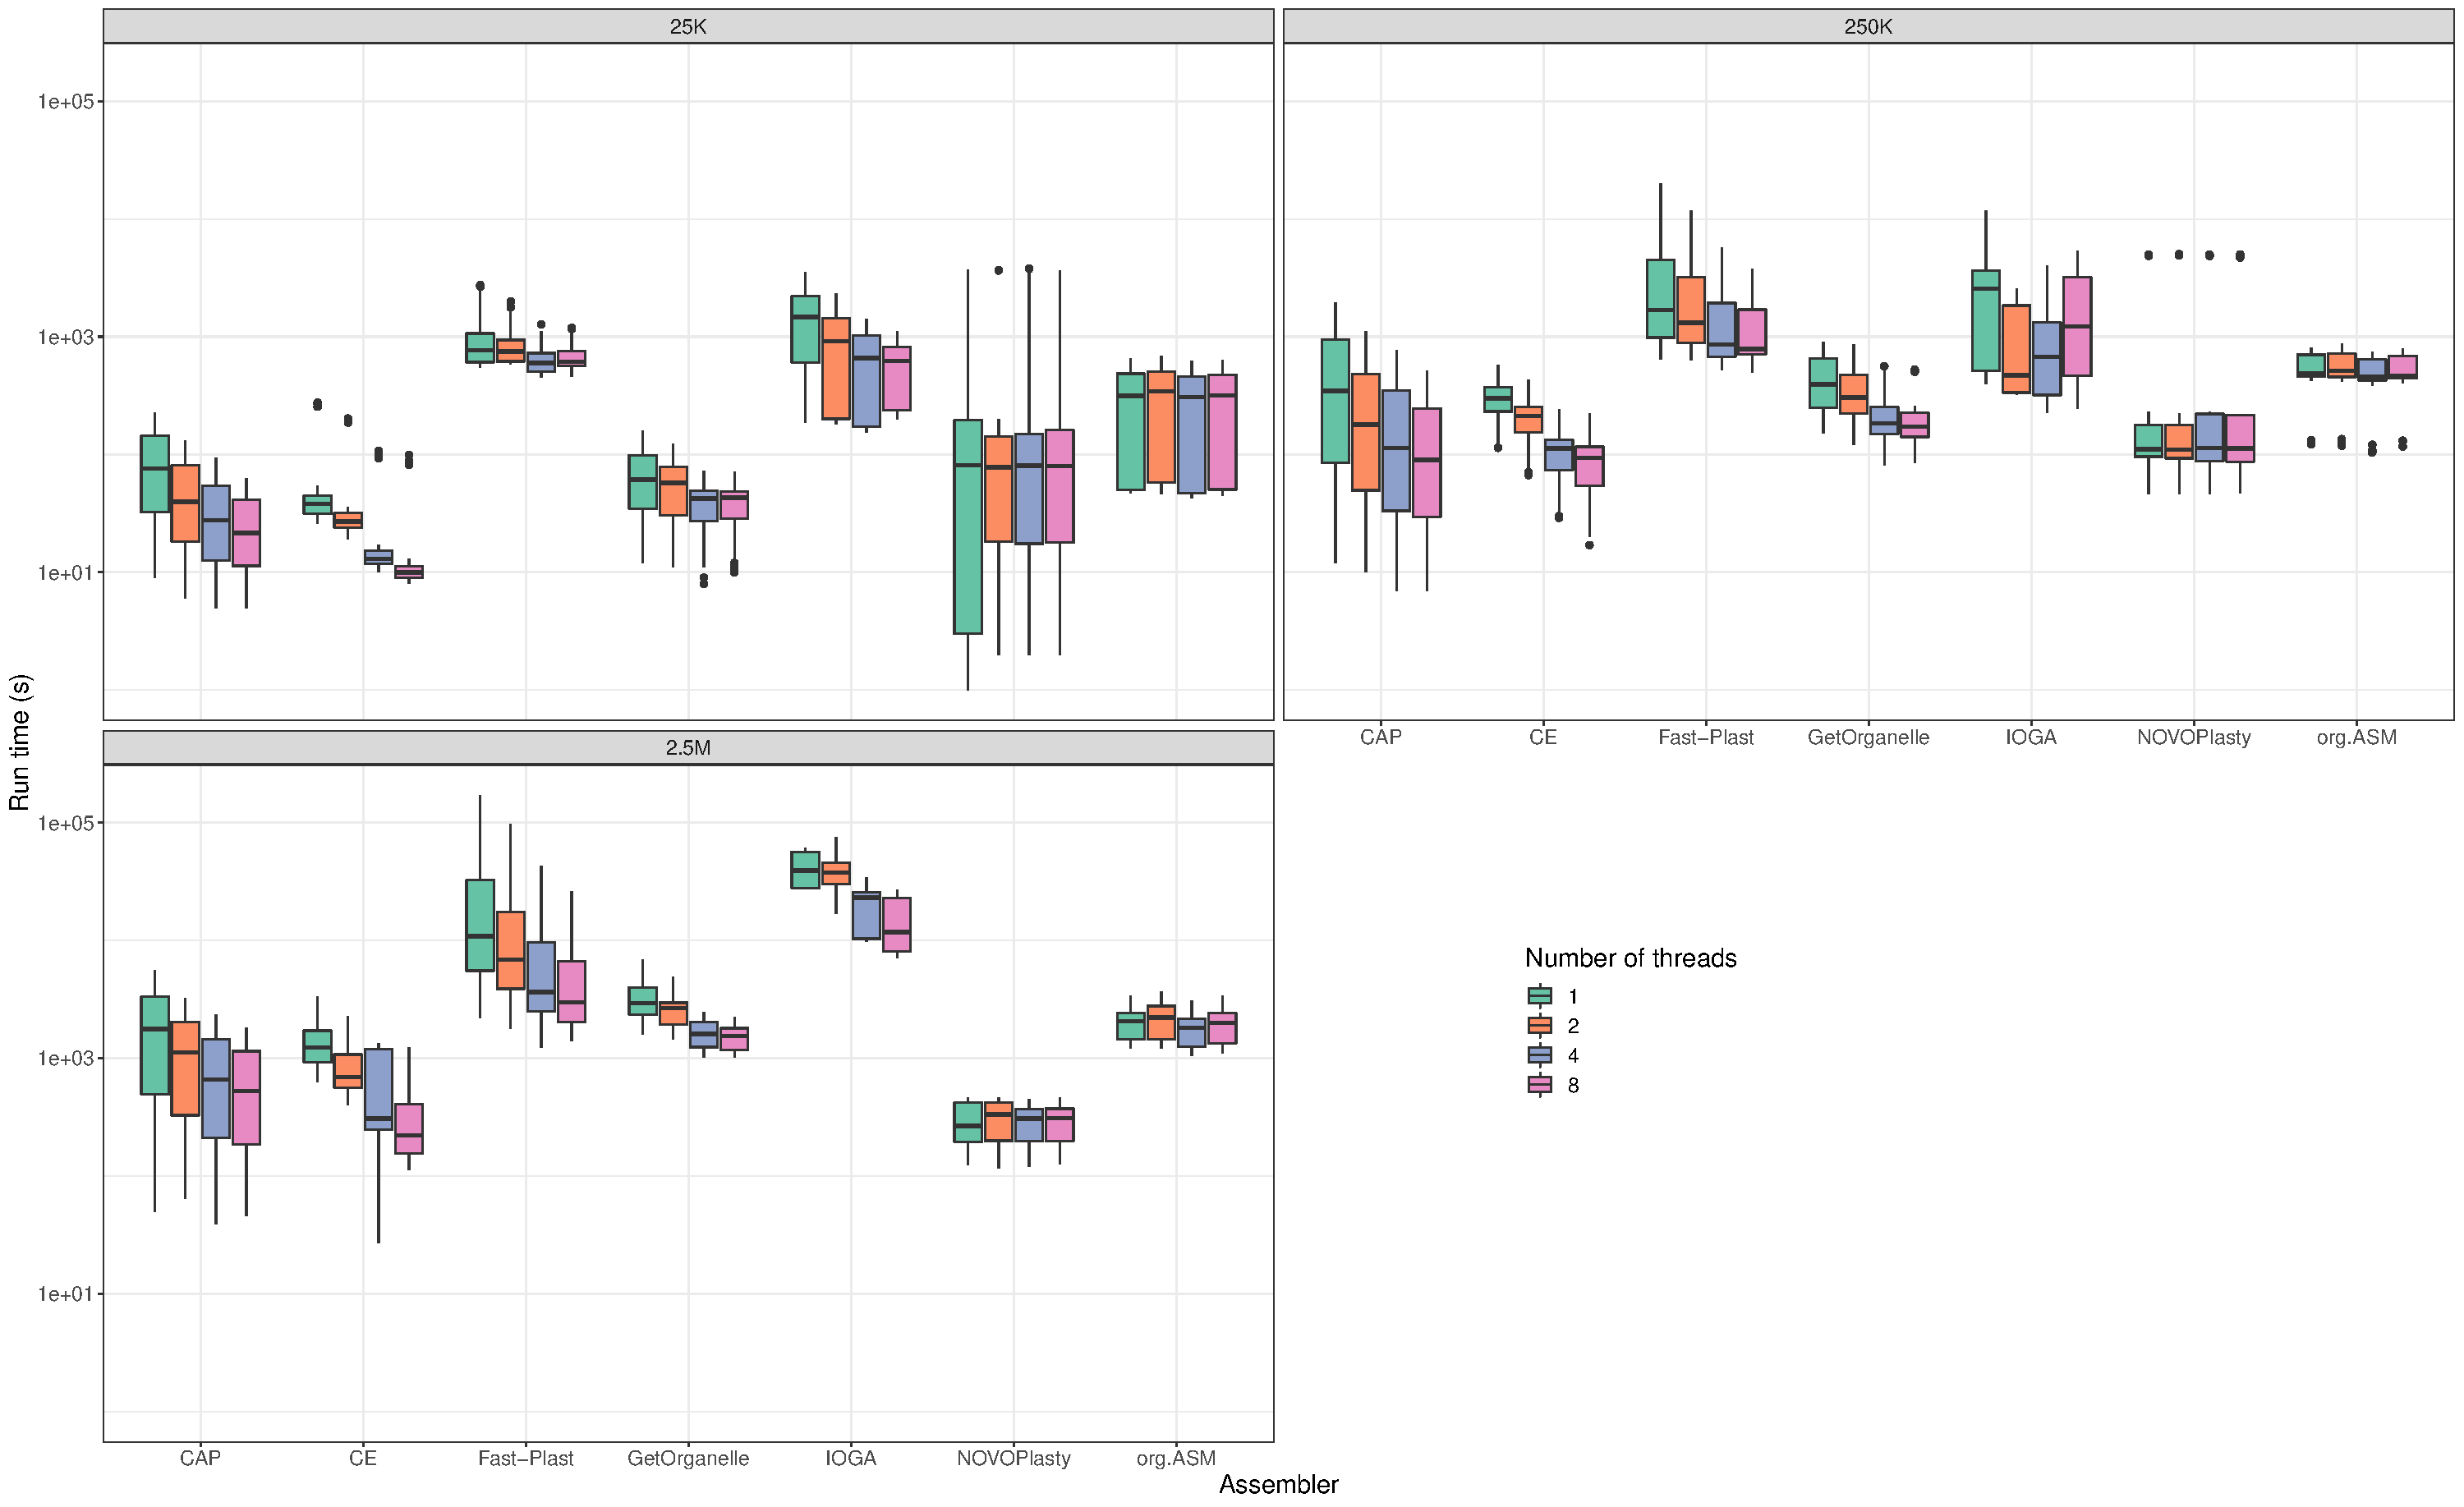
\includegraphics[width=\textwidth]{plots/comp_time_log.pdf}
  \caption{\csentence{Computation time depending on number of threads and size of input data}
  The boxplots show the differences in demand of CPU time for different number of threads and input data size for the seven different assemblers
  }
        \label{fig:performance_runtime}
      \end{figure}

\begin{figure}[h!]
  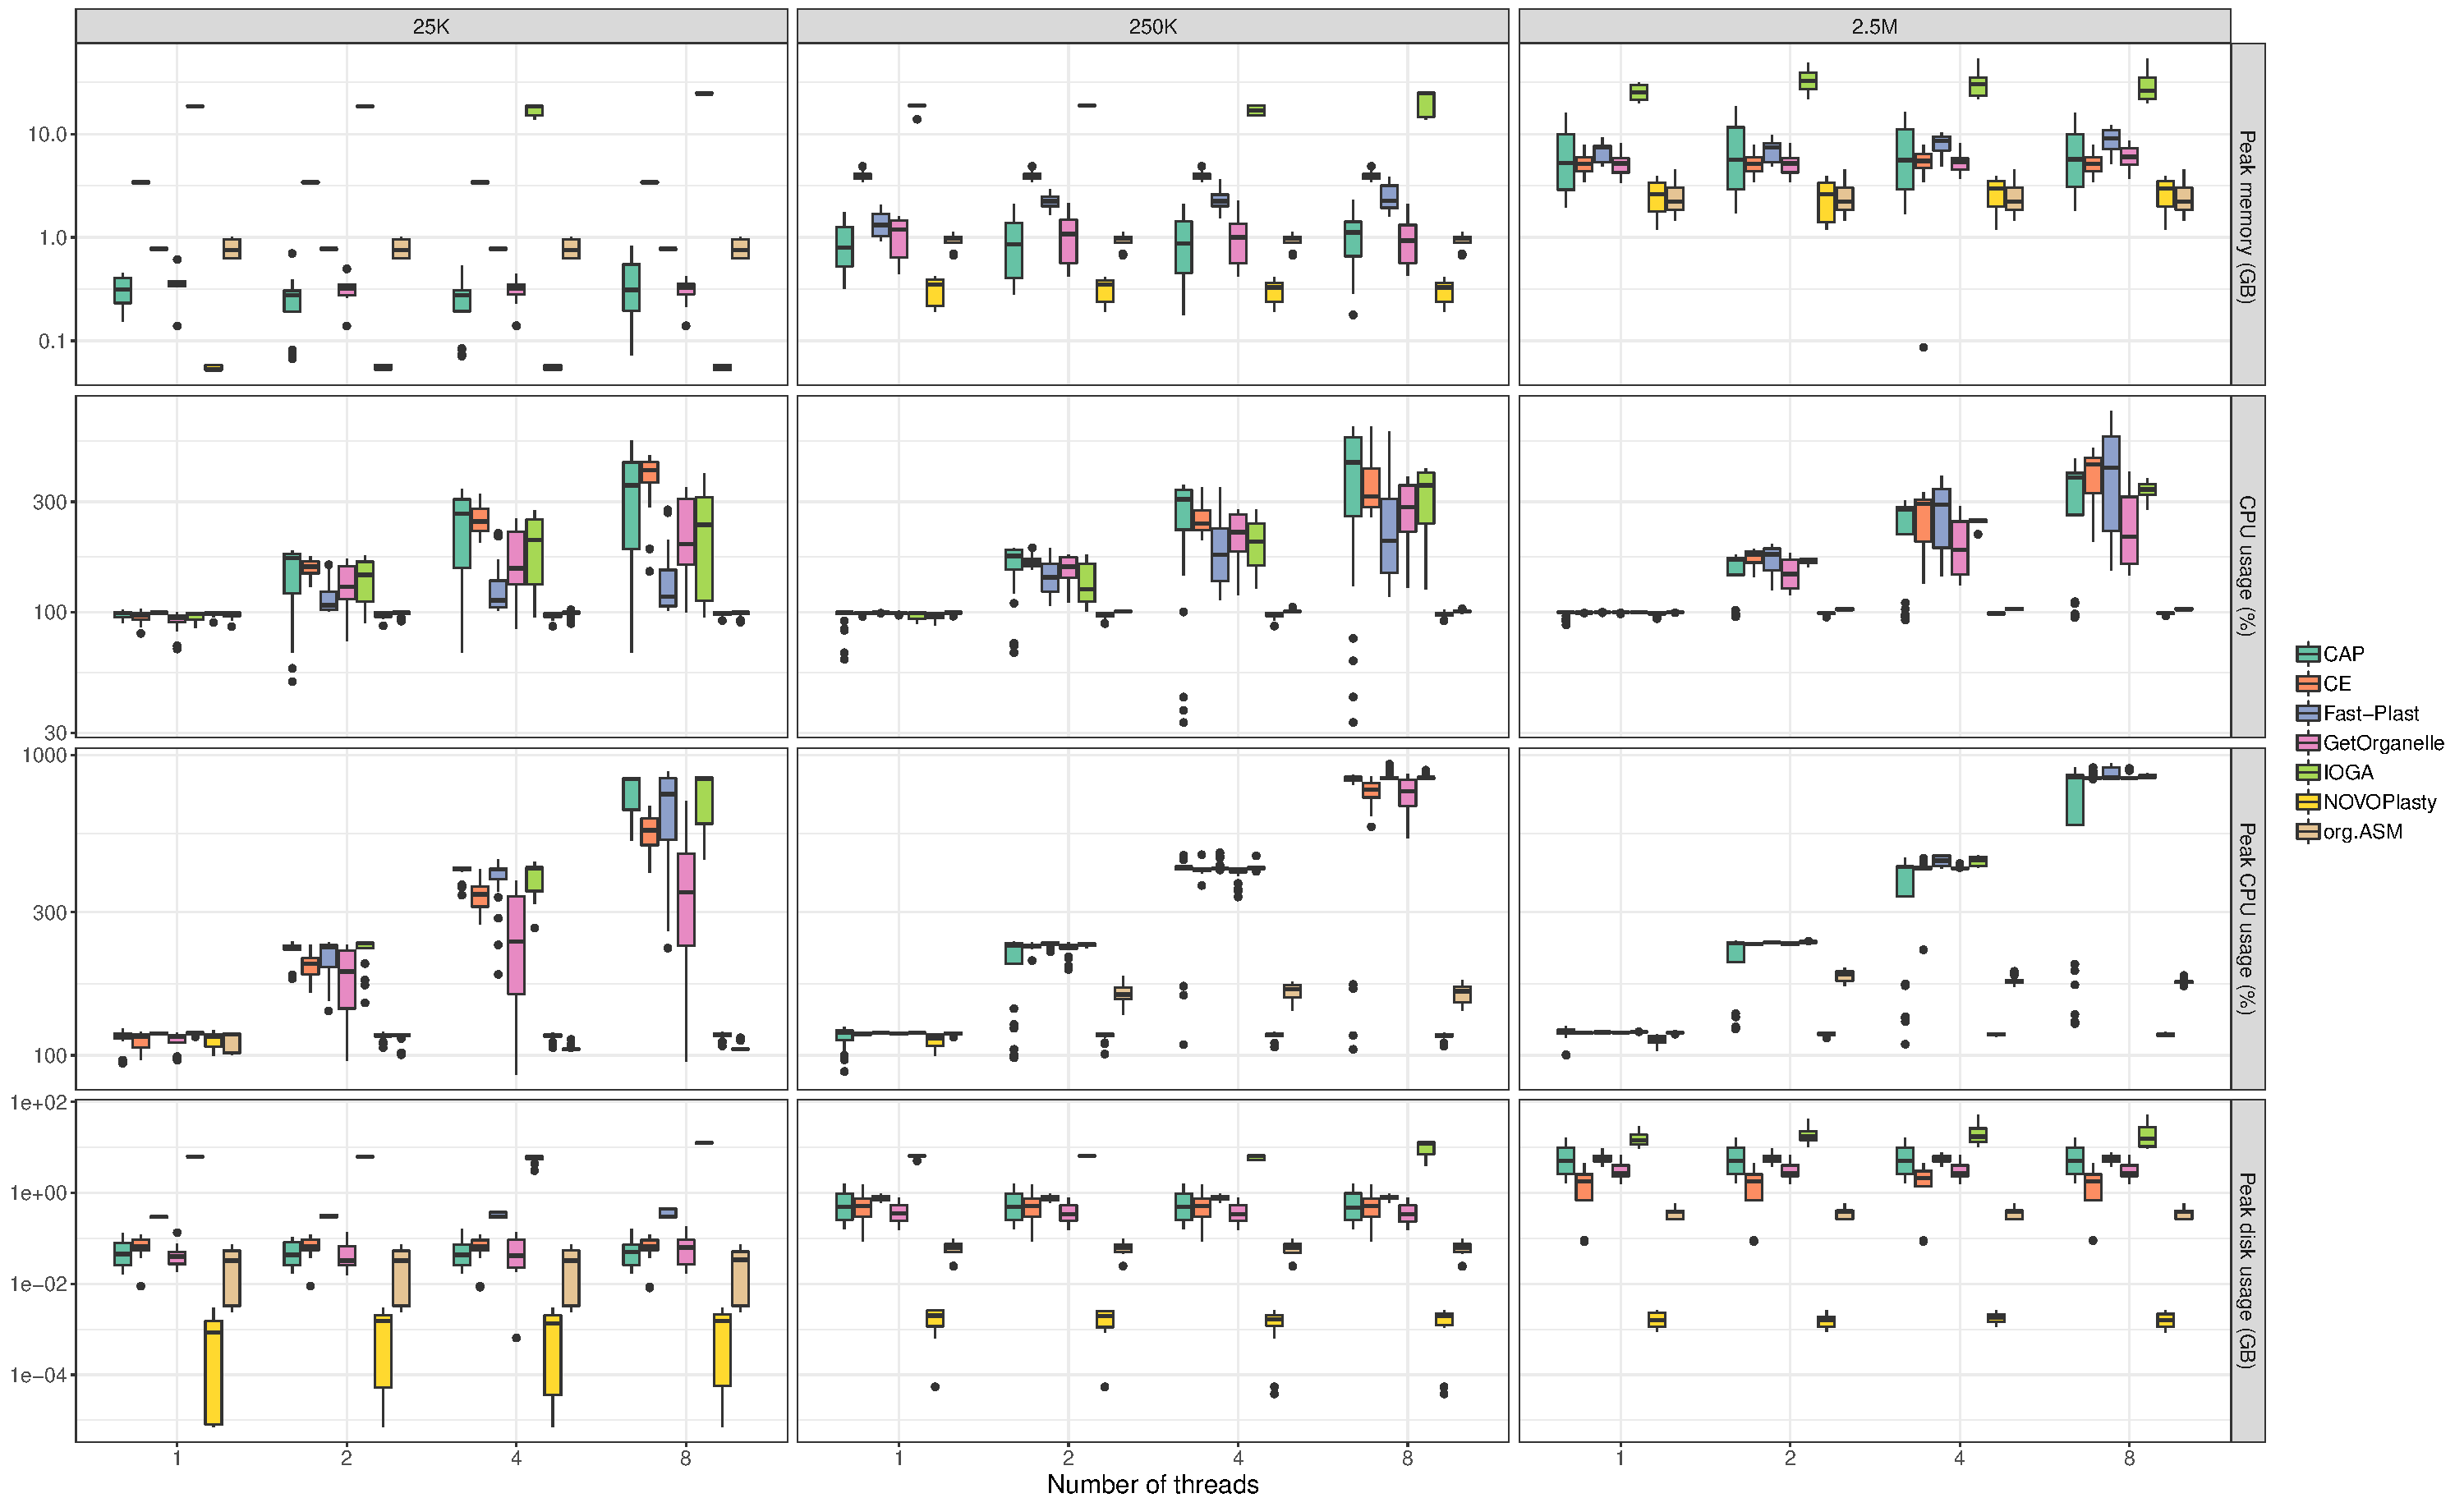
\includegraphics[width=\textwidth]{plots/usage_amount_threads.pdf}
  \caption{\csentence{Performance metrics}
      Boxplots depicting the demand of CPU and RAM and disk space needed depending on the assembler, input data size and number of threads}
      \label{fig:performance_memory_cpu}
      \end{figure}

\begin{figure}[h!]
  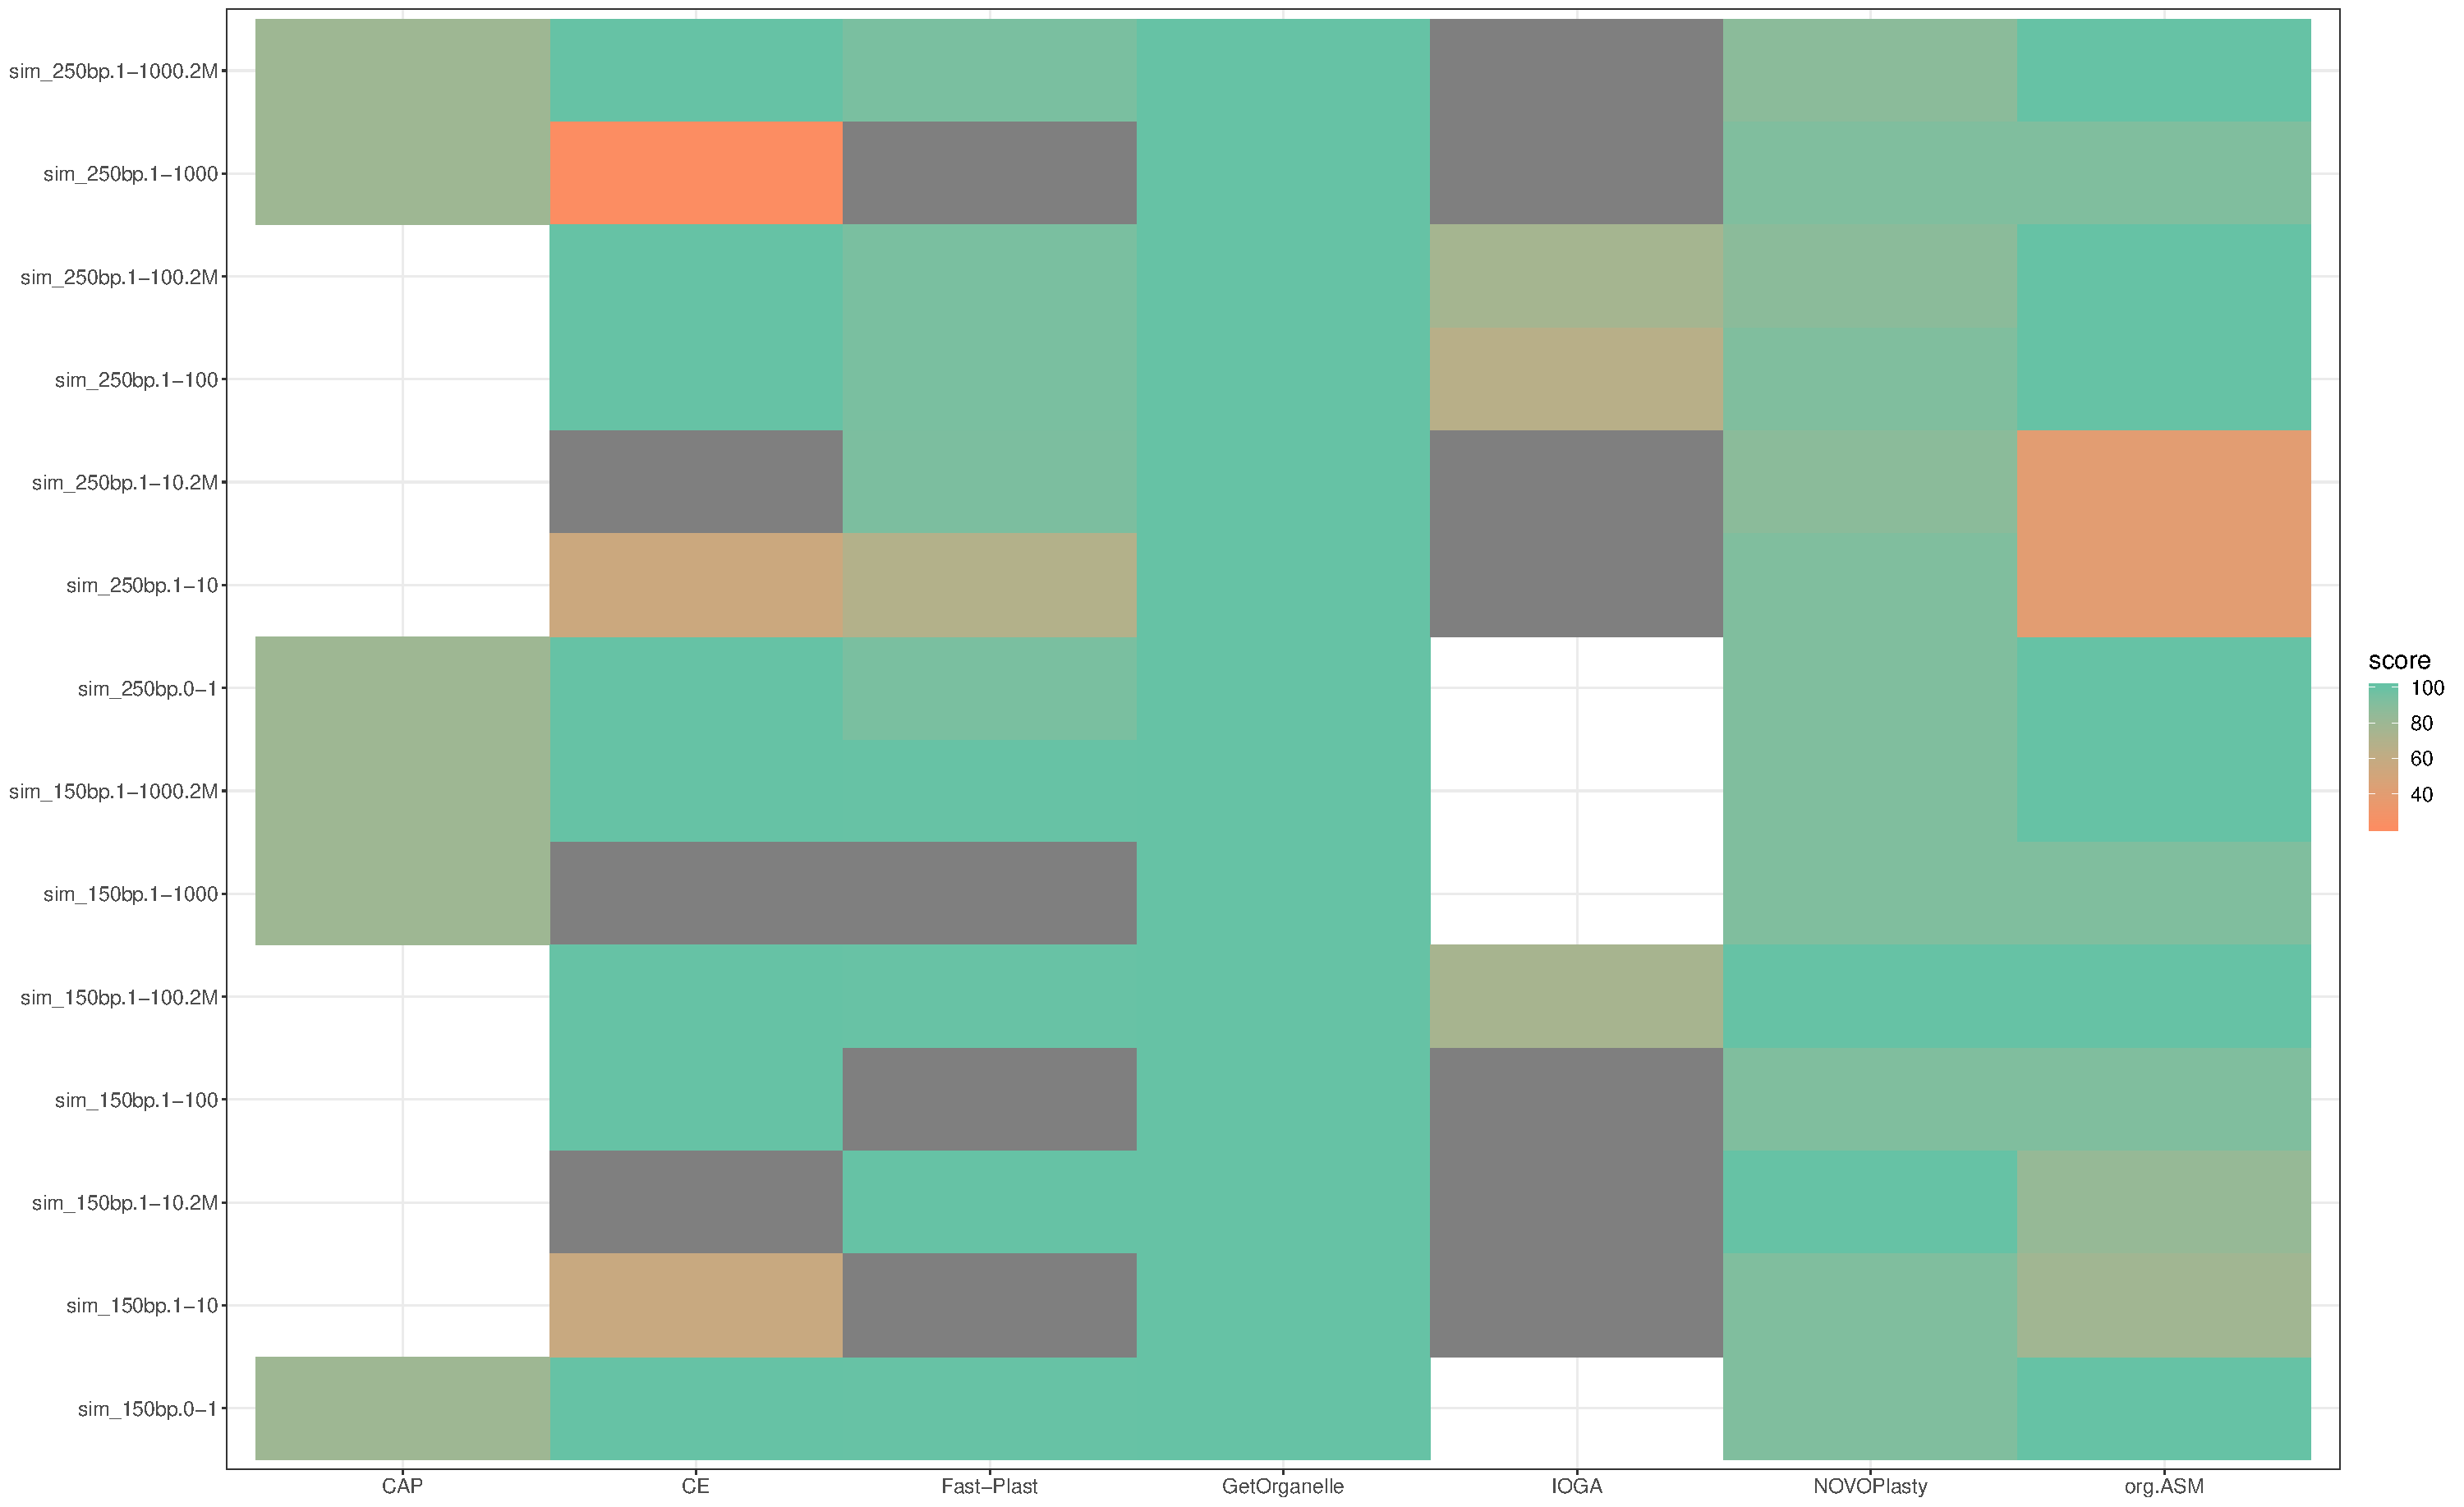
\includegraphics[width=\textwidth]{plots/sim_tiles.pdf}
  \caption{\csentence{Score of assemblies on simulated data}
      Results of assemblies from simulated data sets. Color scale of the tiles represents the score }
      \label{fig:simulated}
      \end{figure}

  \begin{figure}[h!]
  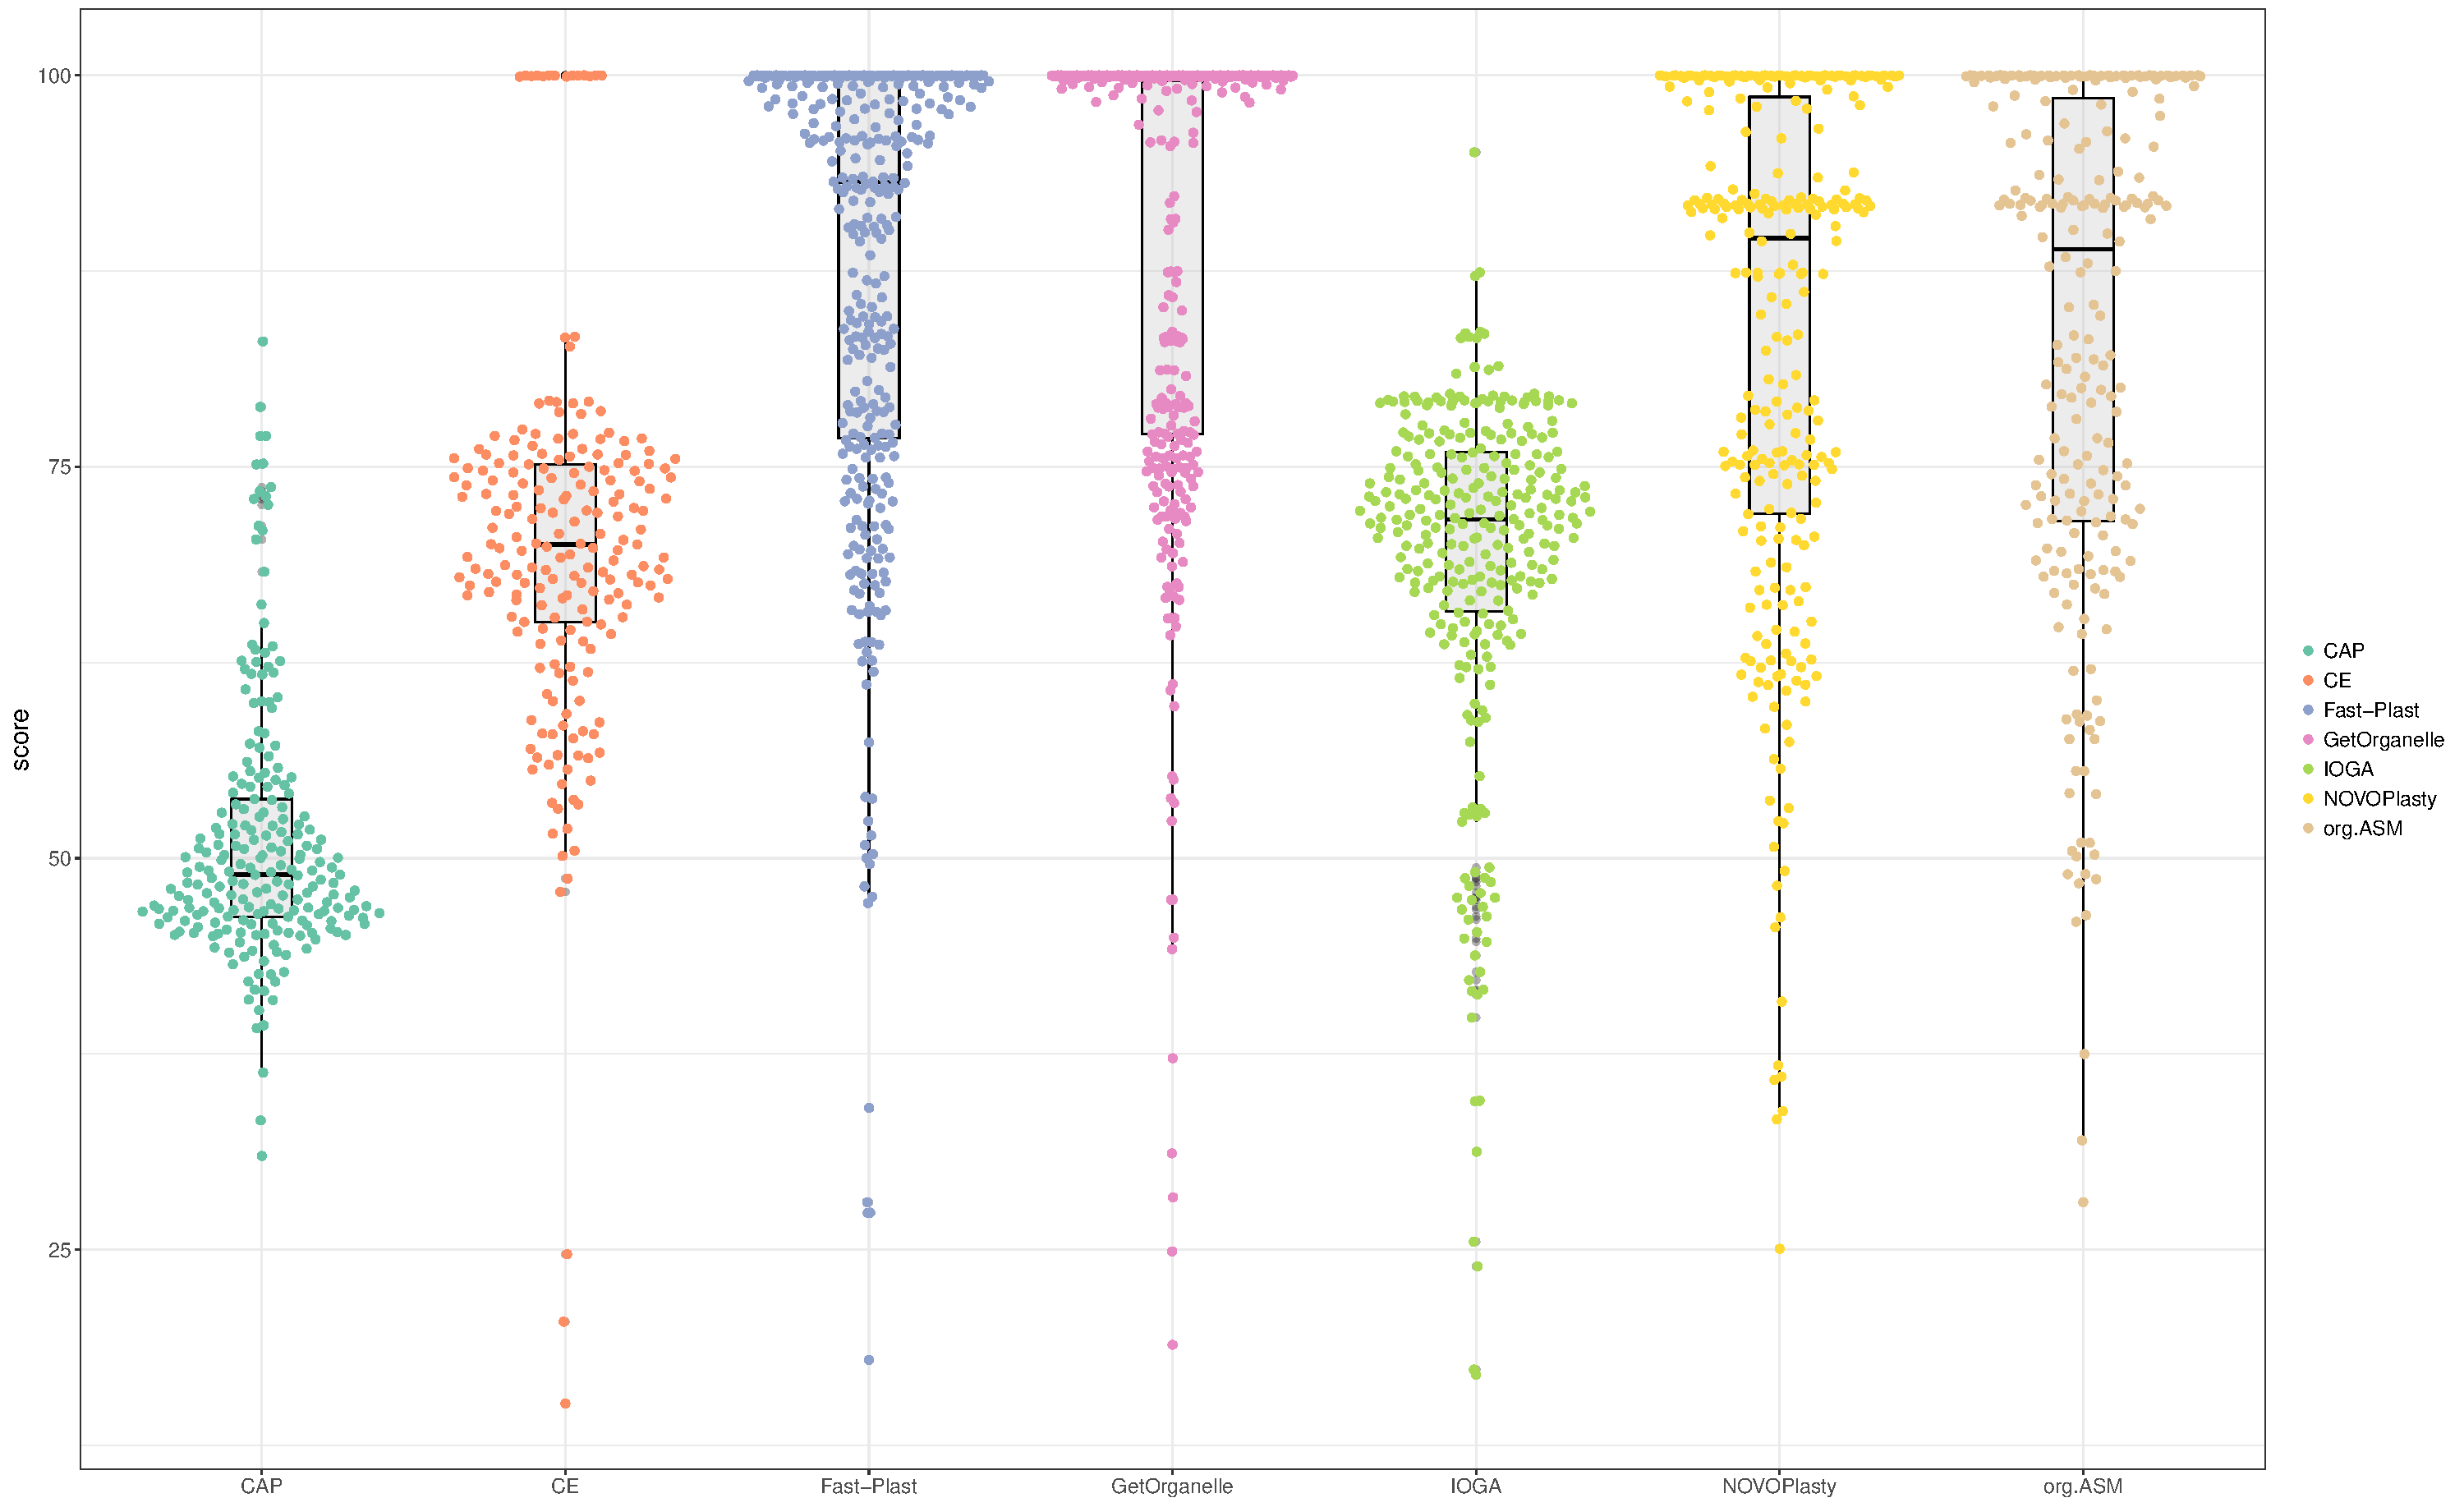
\includegraphics[width=\textwidth]{plots/swarm.pdf}
  \caption{\csentence{Results of scoring of the seven assemblers}
  The box- and swarplots depict the results of the scoring algorithm we used. For the different assemblers. The whiskers of boxplots indicate the 1.5 x interquartile range. 
    }
      \label{fig:swarmplot}
      \end{figure}

\begin{figure}[h!]
  
\includegraphics[width=\textwidth,page=2]{plots/upset.pdf}
  \caption{\csentence{Upset plot \cite{lex2014upset} comparing success of assemblers on the real data sets}
      The plot shows the intersection of success ($score > 99$) between assemblers. For \num{69} data sets only \go{} was able to obtain a complete chloroplast. \num{43} were successful with both \go{} and \fp{} and so on}
            \label{fig:upset}
      \end{figure}

\begin{figure}[h!]
  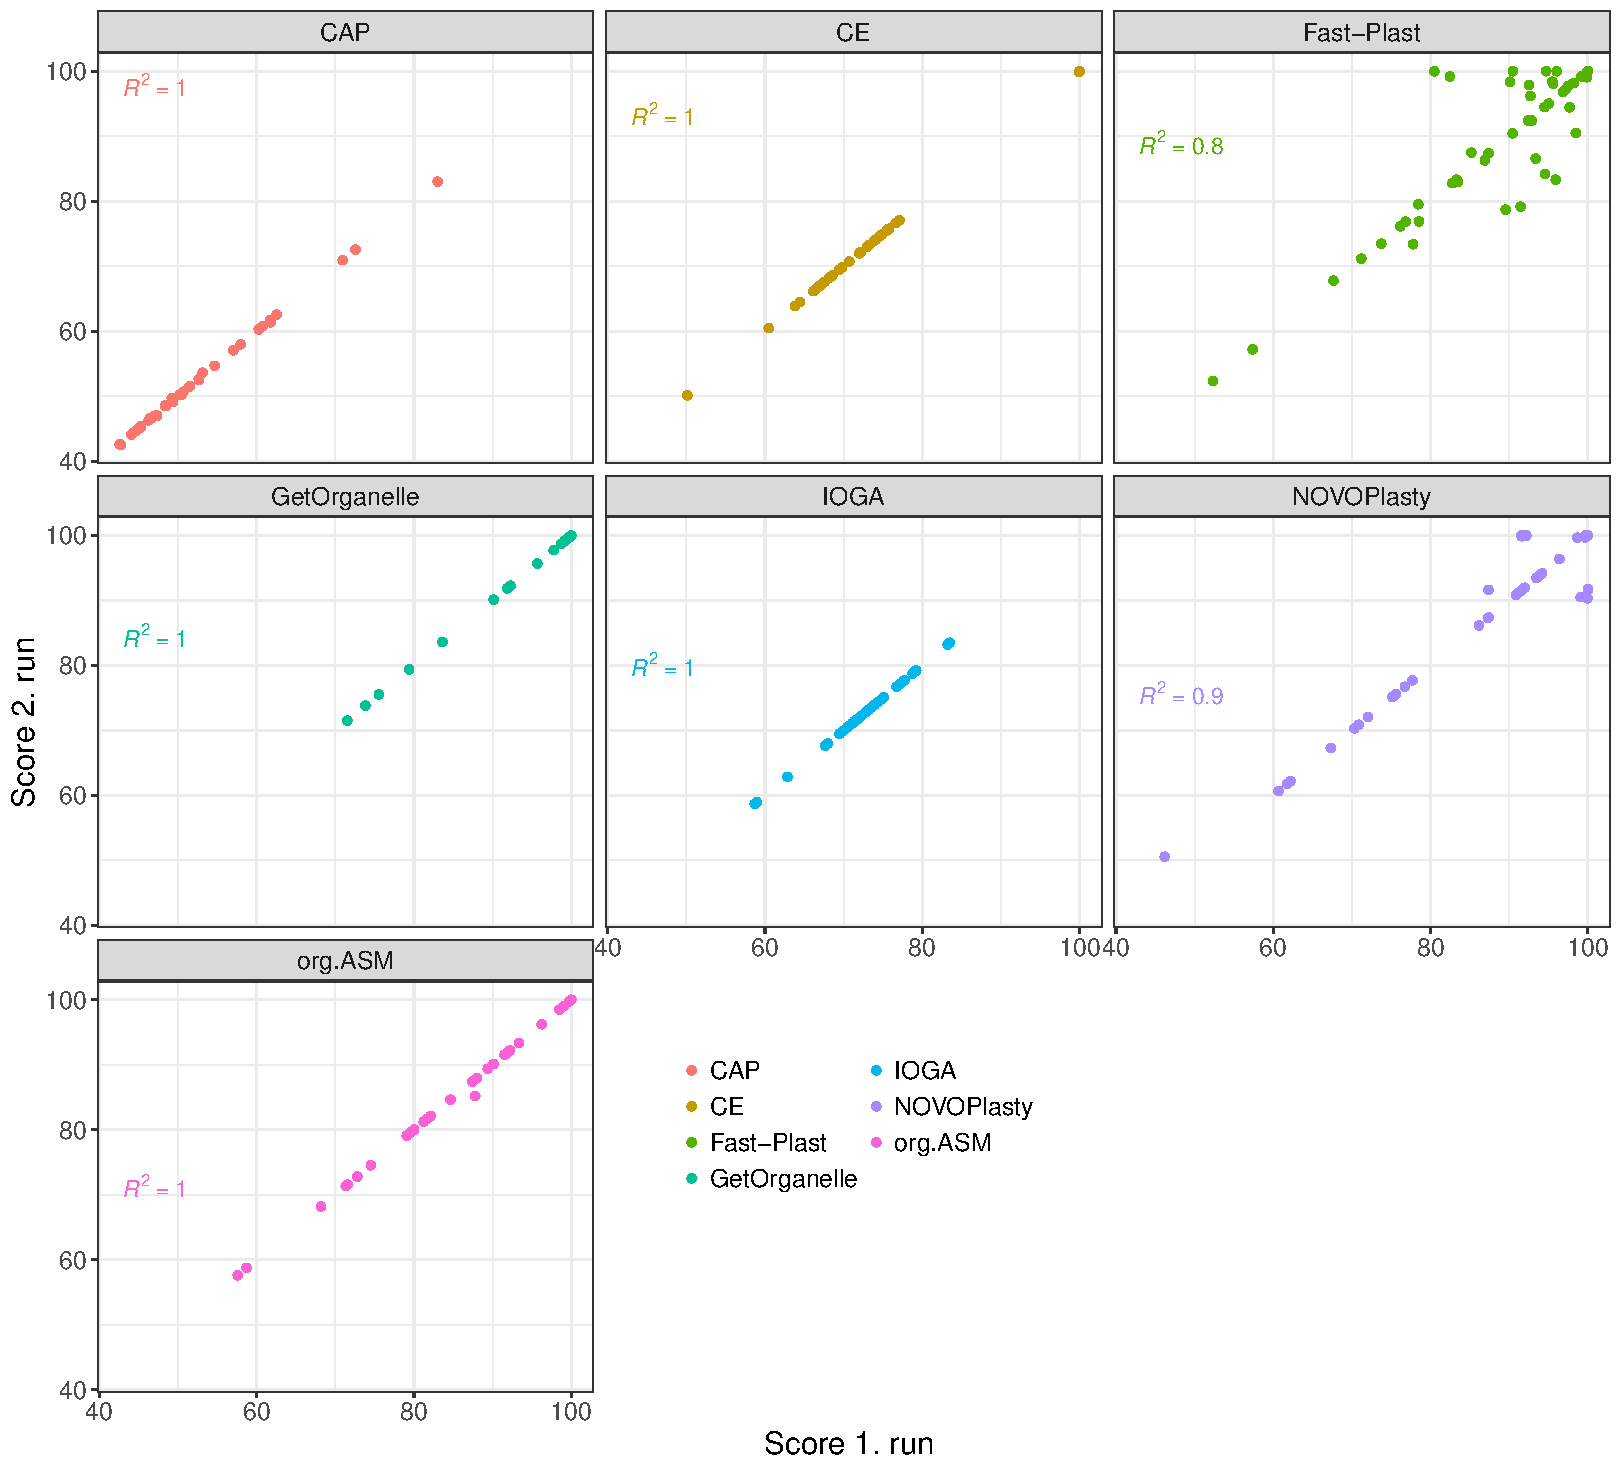
\includegraphics[width=\textwidth]{plots/repro.pdf}
  \caption{\csentence{Scores between two repeated runs for consistency testing}
  The scatter plots depicts the scores of the 1. runs x-axis versus the scores of the 2. run y-axis of the data sets that were selected for re-evaluation. 
      }
      \label{fig:consistency}
      \end{figure}

\begin{figure}[h!]
  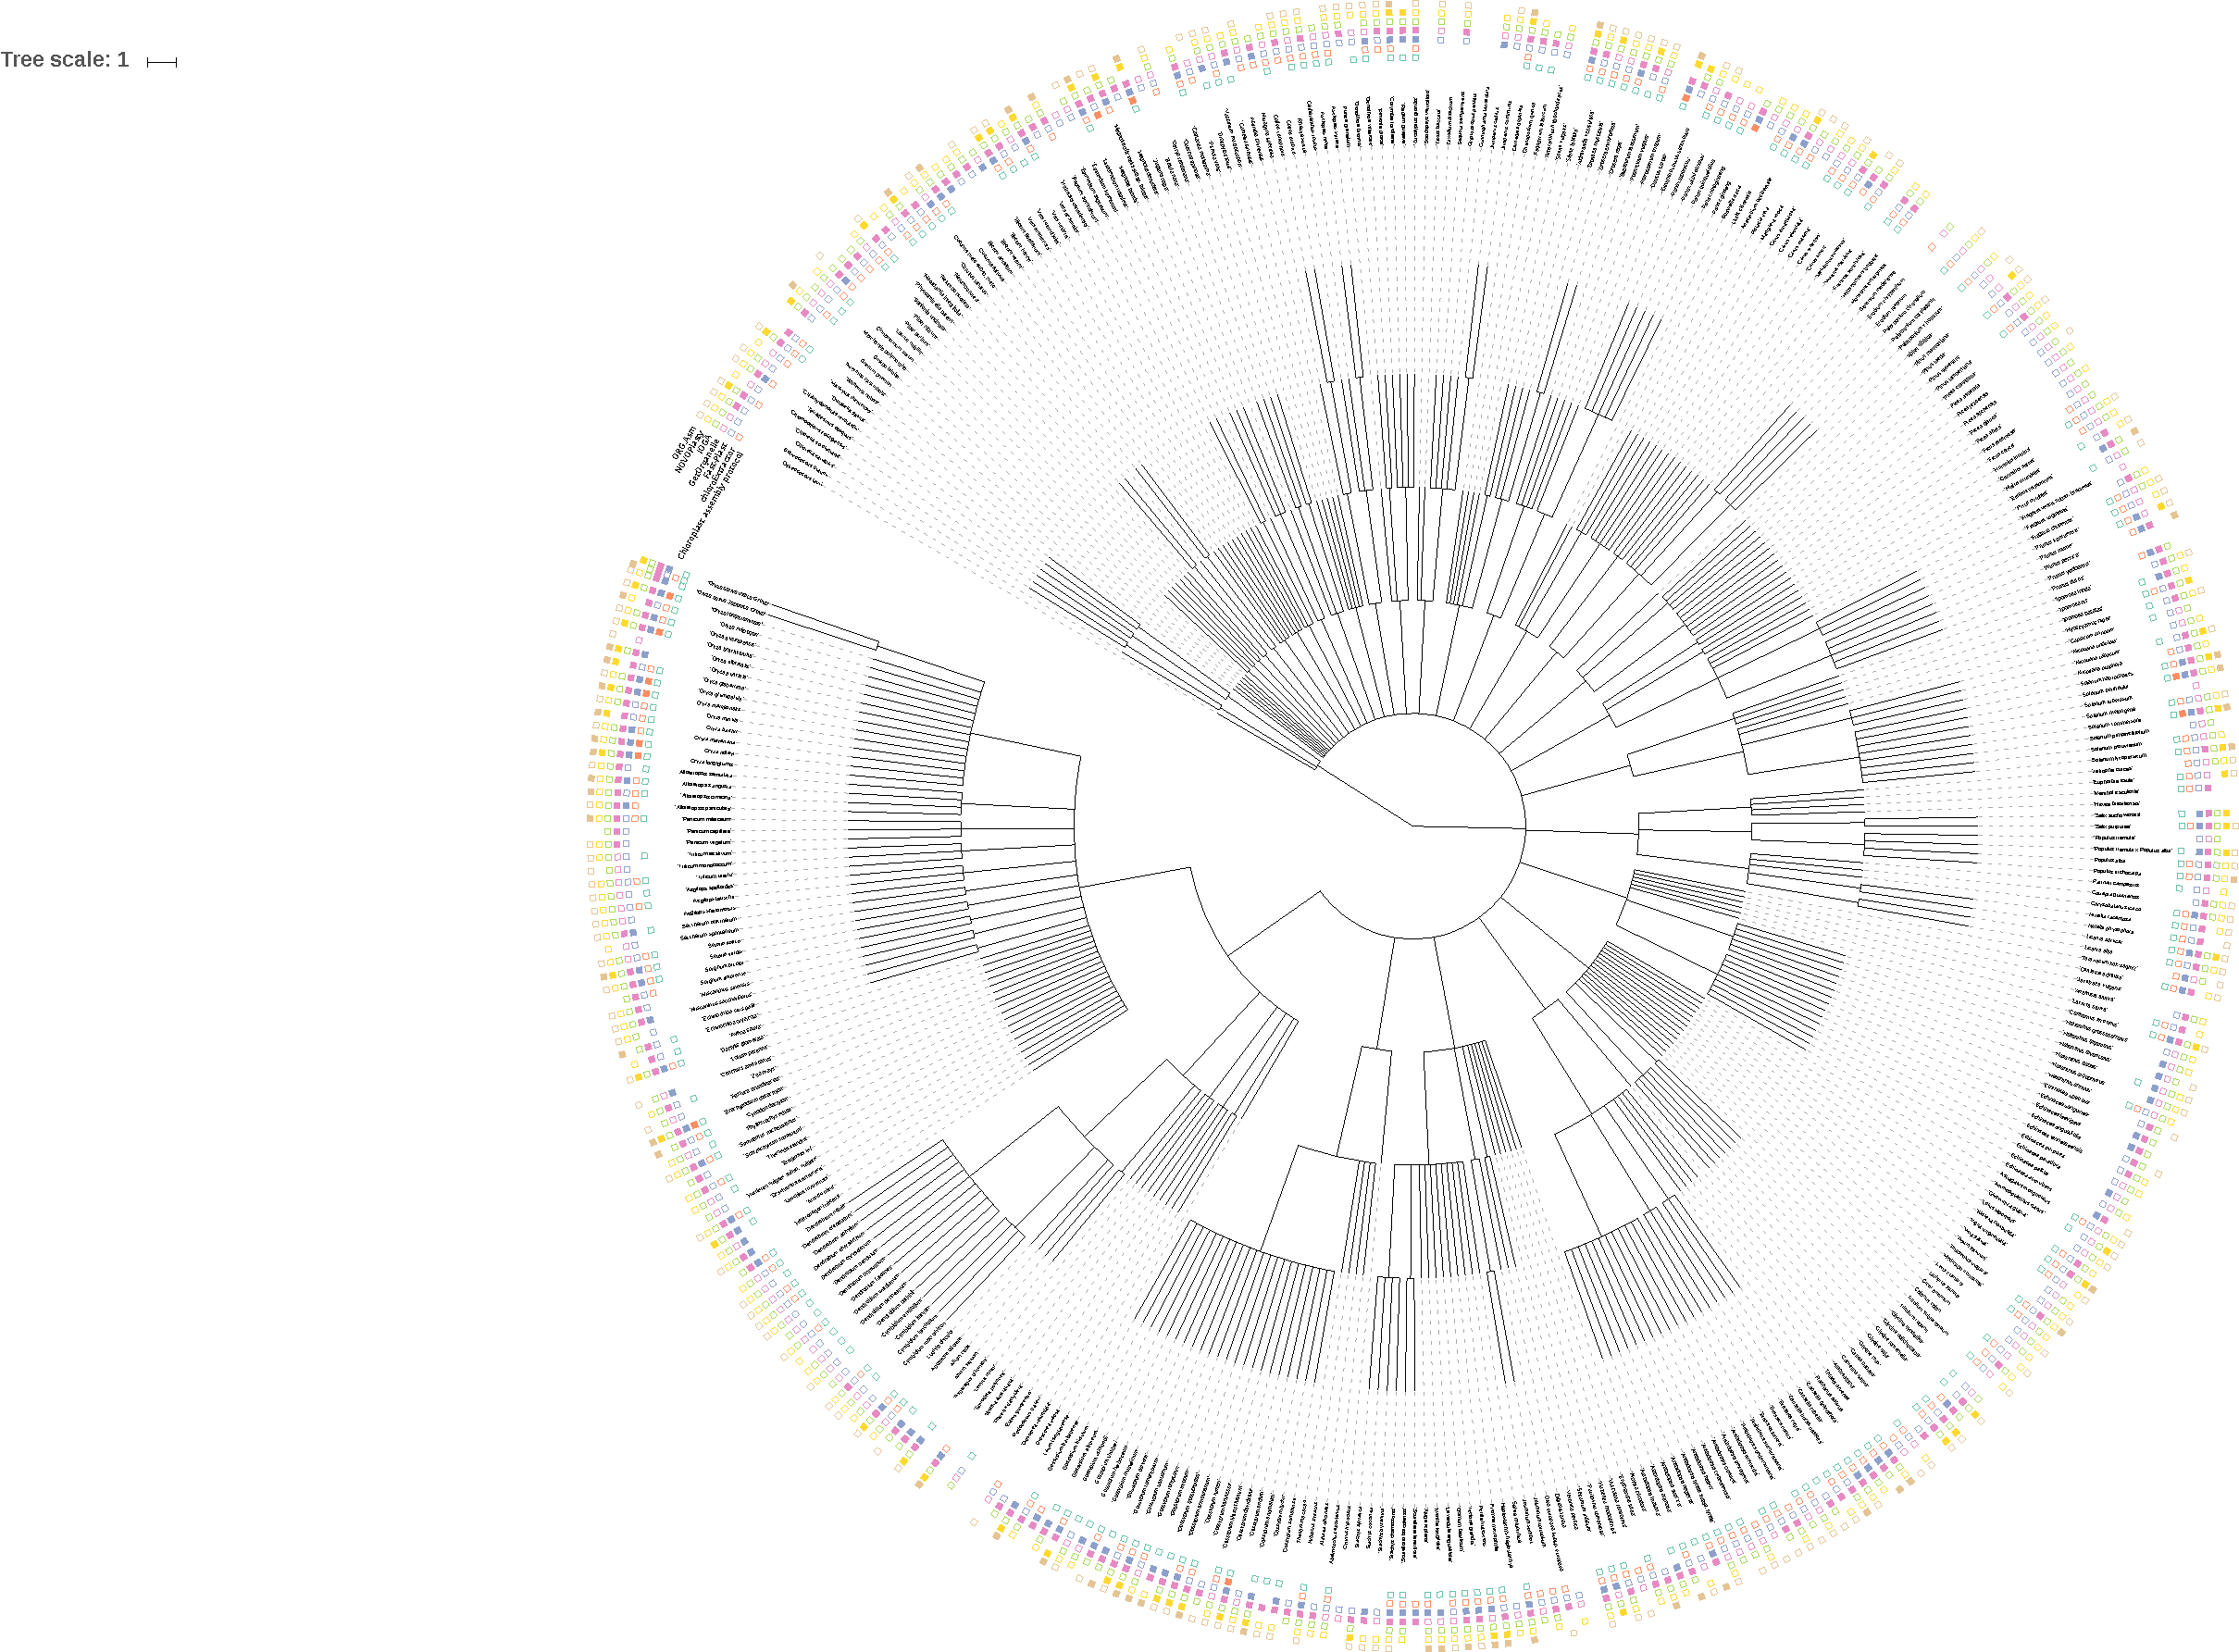
\includegraphics[width=\textwidth]{plots/real_datasets_tree.pdf}
  \caption{\csentence{Success of assemblers on real data sets on tree derived from NCBI taxonomy \cite{ncbi2011}}
       }
      \label{fig:tree}
      \end{figure}\todo{cite itol}

%%%%%%%%%%%%%%%%%%%%%%%%%%%%%%%%%%%
%%                               %%
%% Tables                        %%
%%                               %%
%%%%%%%%%%%%%%%%%%%%%%%%%%%%%%%%%%%

%% Use of \listoftables is discouraged.
%%
\section*{Tables}
\begin{table}[h!]
\caption{Docker images used in our benchmark setup.}
\label{tab:dockerimages}
\centering
      \resizebox{\textwidth}{!}{\begin{tabular}{ccc}
        \hline
          Tool & Image name and tag & SHA256 Checksum   \\ \hline
          \ce & \dockerce & \dockercesha \\
          \cassp & \dockercassp & \dockercasspsha \\
          \fp & \dockerfp & \dockerfpsha \\
          \go & \dockergo & \dockergosha \\
          \ioga & \dockerioga & \dockeriogasha \\
          \np & \dockernp & \dockernpsha \\
          \oa & \dockeroa & \dockeroasha \\ \hline
      \end{tabular}}
\end{table}

\begin{table}[]
    \centering
    \caption{Overview of the results of the qualitative usability evaluation. Each tool 
    could score \good{}, \ok{} or \bad{} in each of the categories.}
    \label{tab:resultsqual}
\begin{tabular}{p{3cm}cccccc}   
Tool & Installation & Test/Tutorial & Documentation & Maintenance & FLOSS\\                           \hline \ce{}     &  \good{}  &  \good{}  &  \good{}  &  \good{}  &  \good{} \\
\cassp{}  &  \ok{}    &  \good{}  &  \ok{}    &  \good{}  &  \good{} \\
\fp{}     &  \bad{}   &  \ok{}    &  \good{}  &  \good{}  &  \good{} \\
\go{}     &  \ok{}    &  \ok{}    &  \good{}  &  \good{}  &  \good{} \\
\ioga{}   &  \bad{}   &  \bad{}   &  \ok{}    &  \ok{}    &  \bad{}  \\
\np{}     &  \good{}  &  \good{}  &  \good{}  &  \good{}  &  \ok{}   \\
\oa{}     &  \bad{}   &  \bad{}   &  \ok{}    &  \good{}  &  \good{} \\ \hline
\end{tabular}      
\end{table}

\begin{table}[ht]
\caption{Scores of assemblies of simulated data}
\label{tab:scores}
\centering
\begin{tabular}{rlrrrrrrr}
  \hline
 & data set & CAP & CE & Fast-Plast & GetOrganelle & IOGA & NOVOPlasty & org.ASM \\ 
  \hline
1 & sim\_150bp.0-1 & 79.10 & 100.00 & 99.72 & 100.00 &  & 91.52 & 100.00 \\ 
  2 & sim\_150bp.1-10 &  & 56.44 &  & 100.00 &  & 91.52 & 78.00 \\ 
  3 & sim\_150bp.1-10.2M &  &  & 99.97 & 100.00 &  & 100.00 & 82.72 \\ 
  4 & sim\_150bp.1-100 &  & 100.00 &  & 100.00 &  & 91.52 & 91.50 \\ 
  5 & sim\_150bp.1-100.2M &  & 100.00 & 99.47 & 100.00 & 74.82 & 100.00 & 100.00 \\ 
  6 & sim\_150bp.1-1000 & 79.10 &  &  & 100.00 &  & 91.52 & 91.50 \\ 
  7 & sim\_150bp.1-1000.2M & 79.10 & 100.00 & 99.72 & 100.00 &  & 91.52 & 100.00 \\ 
  8 & sim\_250bp.0-1 & 79.10 & 100.00 & 93.83 & 100.00 &  & 91.52 & 100.00 \\ 
  9 & sim\_250bp.1-10 &  & 54.98 & 68.45 & 100.00 &  & 91.52 & 40.20 \\ 
  10 & sim\_250bp.1-10.2M &  &  & 93.00 & 100.00 &  & 87.40 & 40.20 \\ 
  11 & sim\_250bp.1-100 &  & 100.00 & 93.83 & 100.00 & 65.81 & 91.52 & 100.00 \\ 
  12 & sim\_250bp.1-100.2M &  & 100.00 & 93.83 & 100.00 & 75.73 & 87.40 & 100.00 \\ 
  13 & sim\_250bp.1-1000 & 79.10 & 21.30 &  & 100.00 &  & 91.52 & 91.50 \\ 
  14 & sim\_250bp.1-1000.2M & 79.10 & 100.00 & 93.83 & 100.00 &  & 87.40 & 100.00 \\ 
   \hline
\end{tabular}
\end{table}


\begin{table}[ht]
\caption{Mean scores of chloroplast genome assemblers}
\label{tab:scores}
\centering
\begin{tabular}{rlrrrr}
  \hline
 & assembler & Mean & SD & N\_perfect & N\_tot \\ 
  \hline
  1 & CAP & 51.26 & 8.42 &   0 & 221 \\ 
  2 & CE & 69.99 & 12.33 &  14 & 205 \\ 
  3 & Fast-Plast & 86.96 & 15.33 & 114 & 352 \\ 
  4 & GetOrganelle & 89.13 & 15.30 & 199 & 356 \\ 
  5 & IOGA & 68.74 & 11.69 &   0 & 296 \\ 
  6 & NOVOPlasty & 82.78 & 16.55 &  66 & 270 \\ 
  7 & org.ASM & 82.77 & 16.38 &  55 & 228 \\ 
   \hline
\end{tabular}
\end{table}



% latex table generated in R 3.6.0 by xtable 1.8-4 package
% Wed May 29 19:46:12 2019
\begin{table}[ht]
\centering
\begin{tabular}{rll}
  \hline
 & V1 & Re-eval \\ 
  \hline
1 & DRR000604 & Yes \\ 
  2 & DRR001794 & NO \\ 
  3 & DRR013917 & NO \\ 
  4 & DRR014074 & NO \\ 
  5 & DRR014095 & NO \\ 
  6 & DRR019500 & Yes \\ 
  7 & DRR022700 & Yes \\ 
  8 & DRR032042 & Yes \\ 
  9 & DRR053294 & Yes \\ 
  10 & DRR054584 & Yes \\ 
  11 & DRR056658 & Yes \\ 
  12 & DRR056663 & Yes \\ 
  13 & DRR056670 & NO \\ 
  14 & DRR056675 & Yes \\ 
  15 & DRR056778 & NO \\ 
  16 & DRR057991 & Yes \\ 
  17 & DRR058012 & NO \\ 
  18 & DRR058031 & Yes \\ 
  19 & DRR063110 & NO \\ 
  20 & DRR083750 & Yes \\ 
  21 & DRR098098 & NO \\ 
  22 & ERR1397263 & Yes \\ 
  23 & ERR1449077 & NO \\ 
  24 & ERR1638191 & Yes \\ 
  25 & ERR1683652 & NO \\ 
  26 & ERR1727007 & NO \\ 
  27 & ERR1735493 & Yes \\ 
  28 & ERR1735613 & NO \\ 
  29 & ERR1735633 & Yes \\ 
  30 & ERR1795324 & Yes \\ 
  31 & ERR2026268 & NO \\ 
  32 & ERR246536 & NO \\ 
  33 & ERR268415 & NO \\ 
  34 & ERR268420 & NO \\ 
  35 & ERR268423 & NO \\ 
  36 & ERR268425 & Yes \\ 
  37 & ERR268429 & NO \\ 
  38 & ERR2696316 & Yes \\ 
  39 & ERR2696318 & Yes \\ 
  40 & ERR276848 & Yes \\ 
  41 & ERR2799526 & Yes \\ 
  42 & ERR2799530 & Yes \\ 
  43 & ERR2799532 & Yes \\ 
  44 & ERR2799534 & NO \\ 
  45 & ERR2799536 & NO \\ 
  46 & ERR2799539 & NO \\ 
  47 & ERR2799542 & Yes \\ 
  48 & ERR2799543 & NO \\ 
  49 & ERR2799544 & Yes \\ 
  50 & ERR2799546 & Yes \\ 
  51 & ERR3148763 & NO \\ 
  52 & ERR321701 & Yes \\ 
  53 & ERR351509 & NO \\ 
  54 & ERR359708 & NO \\ 
  55 & ERR375848 & NO \\ 
  56 & ERR385916 & Yes \\ 
  57 & ERR413103 & NO \\ 
  58 & ERR413115 & Yes \\ 
  59 & ERR413118 & NO \\ 
  60 & ERR424849 & NO \\ 
  61 & ERR636124 & NO \\ 
  62 & ERR964904 & NO \\ 
  63 & SRR073338 & Yes \\ 
  64 & SRR074949 & Yes \\ 
  65 & SRR091633 & NO \\ 
  66 & SRR1028837 & NO \\ 
  67 & SRR1034659 & NO \\ 
  68 & SRR1049756 & NO \\ 
  69 & SRR1145775 & Yes \\ 
  70 & SRR1158316 & Yes \\ 
  71 & SRR1171700 & NO \\ 
  72 & SRR1174380 & NO \\ 
  73 & SRR1176843 & NO \\ 
  74 & SRR1179645 & NO \\ 
  75 & SRR1179646 & Yes \\ 
  76 & SRR1179648 & Yes \\ 
  77 & SRR1179649 & Yes \\ 
  78 & SRR1179651 & NO \\ 
  79 & SRR1179652 & Yes \\ 
  80 & SRR1179655 & Yes \\ 
  81 & SRR1264539 & NO \\ 
  82 & SRR1265940 & NO \\ 
  83 & SRR1265941 & Yes \\ 
  84 & SRR1265942 & NO \\ 
  85 & SRR1276173 & NO \\ 
  86 & SRR1291239 & Yes \\ 
  87 & SRR1392700 & Yes \\ 
  88 & SRR1405699 & NO \\ 
  89 & SRR1463402 & NO \\ 
  90 & SRR1508428 & NO \\ 
  91 & SRR1508958 & Yes \\ 
  92 & SRR1560932 & Yes \\ 
  93 & SRR1612828 & NO \\ 
  94 & SRR1653109 & NO \\ 
  95 & SRR1660449 & NO \\ 
  96 & SRR1686960 & Yes \\ 
  97 & SRR1705621 & NO \\ 
  98 & SRR1735356 & NO \\ 
  99 & SRR1771524 & Yes \\ 
  100 & SRR1771538 & NO \\ 
  101 & SRR1927951 & NO \\ 
  102 & SRR1951920 & NO \\ 
  103 & SRR1982881 & Yes \\ 
  104 & SRR2012721 & NO \\ 
  105 & SRR2012734 & NO \\ 
  106 & SRR2026990 & Yes \\ 
  107 & SRR2040775 & Yes \\ 
  108 & SRR2040802 & NO \\ 
  109 & SRR2040807 & Yes \\ 
  110 & SRR2040810 & NO \\ 
  111 & SRR2040831 & Yes \\ 
  112 & SRR2054762 & Yes \\ 
  113 & SRR2057822 & Yes \\ 
  114 & SRR2057910 & NO \\ 
  115 & SRR2082664 & Yes \\ 
  116 & SRR2084154 & NO \\ 
  117 & SRR2120220 & Yes \\ 
  118 & SRR2154065 & NO \\ 
  119 & SRR2155086 & NO \\ 
  120 & SRR2518264 & NO \\ 
  121 & SRR2729212 & Yes \\ 
  122 & SRR2847384 & Yes \\ 
  123 & SRR3089810 & NO \\ 
  124 & SRR3138168 & Yes \\ 
  125 & SRR3170741 & NO \\ 
  126 & SRR3170744 & Yes \\ 
  127 & SRR3170745 & Yes \\ 
  128 & SRR3170746 & Yes \\ 
  129 & SRR3170747 & NO \\ 
  130 & SRR3204556 & Yes \\ 
  131 & SRR3340908 & NO \\ 
  132 & SRR3399331 & NO \\ 
  133 & SRR3407090 & NO \\ 
  134 & SRR3407098 & NO \\ 
  135 & SRR3484539 & Yes \\ 
  136 & SRR3492253 & NO \\ 
  137 & SRR3560148 & NO \\ 
  138 & SRR3560152 & Yes \\ 
  139 & SRR3560153 & NO \\ 
  140 & SRR3560157 & NO \\ 
  141 & SRR3560160 & Yes \\ 
  142 & SRR3560184 & NO \\ 
  143 & SRR3560187 & Yes \\ 
  144 & SRR3571175 & NO \\ 
  145 & SRR3678826 & Yes \\ 
  146 & SRR3721649 & NO \\ 
  147 & SRR3747540 & Yes \\ 
  148 & SRR384895 & NO \\ 
  149 & SRR3923695 & Yes \\ 
  150 & SRR3927005 & Yes \\ 
  151 & SRR3927127 & NO \\ 
  152 & SRR3927459 & NO \\ 
  153 & SRR3932120 & NO \\ 
  154 & SRR3932122 & Yes \\ 
  155 & SRR3932123 & Yes \\ 
  156 & SRR3932124 & NO \\ 
  157 & SRR3932128 & NO \\ 
  158 & SRR3932135 & Yes \\ 
  159 & SRR3932138 & Yes \\ 
  160 & SRR3932139 & NO \\ 
  161 & SRR3932141 & Yes \\ 
  162 & SRR3932144 & Yes \\ 
  163 & SRR3932147 & Yes \\ 
  164 & SRR3938254 & Yes \\ 
  165 & SRR396657 & NO \\ 
  166 & SRR4010671 & NO \\ 
  167 & SRR4020477 & NO \\ 
  168 & SRR4028761 & Yes \\ 
  169 & SRR4051980 & NO \\ 
  170 & SRR4063259 & Yes \\ 
  171 & SRR4063804 & Yes \\ 
  172 & SRR4128972 & Yes \\ 
  173 & SRR4159530 & Yes \\ 
  174 & SRR4235199 & Yes \\ 
  175 & SRR4240953 & Yes \\ 
  176 & SRR424217 & Yes \\ 
  177 & SRR4292644 & NO \\ 
  178 & SRR4319202 & Yes \\ 
  179 & SRR4428742 & NO \\ 
  180 & SRR4434178 & NO \\ 
  181 & SRR4453367 & Yes \\ 
  182 & SRR485871 & Yes \\ 
  183 & SRR486146 & Yes \\ 
  184 & SRR490932 & NO \\ 
  185 & SRR5028182 & Yes \\ 
  186 & SRR5036293 & NO \\ 
  187 & SRR5073560 & NO \\ 
  188 & SRR5115287 & Yes \\ 
  189 & SRR5183095 & Yes \\ 
  190 & SRR5196234 & Yes \\ 
  191 & SRR5204424 & Yes \\ 
  192 & SRR5217671 & Yes \\ 
  193 & SRR5236602 & NO \\ 
  194 & SRR5307620 & Yes \\ 
  195 & SRR5310953 & Yes \\ 
  196 & SRR5349609 & NO \\ 
  197 & SRR5349620 & NO \\ 
  198 & SRR5349713 & NO \\ 
  199 & SRR5412136 & NO \\ 
  200 & SRR5433722 & Yes \\ 
  201 & SRR5446059 & Yes \\ 
  202 & SRR5457035 & Yes \\ 
  203 & SRR5467392 & NO \\ 
  204 & SRR547959 & NO \\ 
  205 & SRR5533645 & Yes \\ 
  206 & SRR553489 & NO \\ 
  207 & SRR559245 & NO \\ 
  208 & SRR5602572 & NO \\ 
  209 & SRR5602573 & NO \\ 
  210 & SRR5602574 & Yes \\ 
  211 & SRR5602575 & NO \\ 
  212 & SRR5602576 & NO \\ 
  213 & SRR5602577 & Yes \\ 
  214 & SRR5602578 & NO \\ 
  215 & SRR5602579 & Yes \\ 
  216 & SRR5602580 & Yes \\ 
  217 & SRR5602581 & NO \\ 
  218 & SRR5602582 & NO \\ 
  219 & SRR5602583 & NO \\ 
  220 & SRR5602584 & NO \\ 
  221 & SRR5602585 & Yes \\ 
  222 & SRR5602586 & NO \\ 
  223 & SRR5602587 & NO \\ 
  224 & SRR5602588 & NO \\ 
  225 & SRR5602589 & NO \\ 
  226 & SRR5602590 & Yes \\ 
  227 & SRR5602591 & NO \\ 
  228 & SRR5602592 & NO \\ 
  229 & SRR5602593 & NO \\ 
  230 & SRR5602594 & Yes \\ 
  231 & SRR5602595 & Yes \\ 
  232 & SRR5602596 & NO \\ 
  233 & SRR5602597 & NO \\ 
  234 & SRR5602598 & NO \\ 
  235 & SRR5602600 & NO \\ 
  236 & SRR5602601 & NO \\ 
  237 & SRR5602602 & Yes \\ 
  238 & SRR5602603 & Yes \\ 
  239 & SRR5602604 & Yes \\ 
  240 & SRR5602605 & Yes \\ 
  241 & SRR5602606 & Yes \\ 
  242 & SRR5602607 & NO \\ 
  243 & SRR5602608 & NO \\ 
  244 & SRR5602609 & NO \\ 
  245 & SRR5602610 & NO \\ 
  246 & SRR5602611 & NO \\ 
  247 & SRR5627788 & NO \\ 
  248 & SRR5678803 & NO \\ 
  249 & SRR5757713 & NO \\ 
  250 & SRR576525 & NO \\ 
  251 & SRR576529 & NO \\ 
  252 & SRR576531 & NO \\ 
  253 & SRR576532 & Yes \\ 
  254 & SRR576534 & Yes \\ 
  255 & SRR576536 & NO \\ 
  256 & SRR5807695 & Yes \\ 
  257 & SRR5812493 & NO \\ 
  258 & SRR5812494 & NO \\ 
  259 & SRR5812495 & NO \\ 
  260 & SRR5812496 & Yes \\ 
  261 & SRR5812497 & NO \\ 
  262 & SRR5812498 & Yes \\ 
  263 & SRR5812499 & NO \\ 
  264 & SRR5826129 & Yes \\ 
  265 & SRR5891909 & Yes \\ 
  266 & SRR5891950 & NO \\ 
  267 & SRR5893651 & NO \\ 
  268 & SRR5894861 & NO \\ 
  269 & SRR5902661 & Yes \\ 
  270 & SRR5907715 & Yes \\ 
  271 & SRR5907716 & NO \\ 
  272 & SRR5907791 & NO \\ 
  273 & SRR5920285 & NO \\ 
  274 & SRR5938314 & NO \\ 
  275 & SRR6037860 & Yes \\ 
  276 & SRR6048019 & Yes \\ 
  277 & SRR6056489 & NO \\ 
  278 & SRR6117754 & NO \\ 
  279 & SRR6117755 & Yes \\ 
  280 & SRR6117756 & NO \\ 
  281 & SRR6117757 & NO \\ 
  282 & SRR6175451 & NO \\ 
  283 & SRR617704 & Yes \\ 
  284 & SRR6188466 & NO \\ 
  285 & SRR6220521 & NO \\ 
  286 & SRR6334536 & NO \\ 
  287 & SRR6334584 & NO \\ 
  288 & SRR6355713 & NO \\ 
  289 & SRR6440975 & NO \\ 
  290 & SRR6442327 & Yes \\ 
  291 & SRR6490504 & Yes \\ 
  292 & SRR6512791 & NO \\ 
  293 & SRR6512793 & NO \\ 
  294 & SRR6512795 & NO \\ 
  295 & SRR6512796 & Yes \\ 
  296 & SRR6650558 & Yes \\ 
  297 & SRR6667669 & NO \\ 
  298 & SRR6702454 & NO \\ 
  299 & SRR6780757 & NO \\ 
  300 & SRR6796784 & NO \\ 
  301 & SRR6816710 & NO \\ 
  302 & SRR6823488 & NO \\ 
  303 & SRR6856349 & NO \\ 
  304 & SRR6885354 & NO \\ 
  305 & SRR6940033 & NO \\ 
  306 & SRR6940036 & Yes \\ 
  307 & SRR6940062 & NO \\ 
  308 & SRR6940065 & Yes \\ 
  309 & SRR6940083 & Yes \\ 
  310 & SRR6940087 & NO \\ 
  311 & SRR6940088 & Yes \\ 
  312 & SRR7012756 & NO \\ 
  313 & SRR7040334 & NO \\ 
  314 & SRR7072322 & NO \\ 
  315 & SRR7072324 & NO \\ 
  316 & SRR7072766 & NO \\ 
  317 & SRR7072768 & Yes \\ 
  318 & SRR7125688 & Yes \\ 
  319 & SRR7159815 & NO \\ 
  320 & SRR7160359 & NO \\ 
  321 & SRR7285294 & Yes \\ 
  322 & SRR7341625 & Yes \\ 
  323 & SRR7341626 & NO \\ 
  324 & SRR7528994 & Yes \\ 
  325 & SRR7528995 & NO \\ 
  326 & SRR7529014 & Yes \\ 
  327 & SRR7529015 & Yes \\ 
  328 & SRR7548934 & Yes \\ 
  329 & SRR7601255 & Yes \\ 
  330 & SRR7630500 & Yes \\ 
  331 & SRR7637319 & NO \\ 
  332 & SRR7666034 & NO \\ 
  333 & SRR7725010 & Yes \\ 
  334 & SRR7771854 & Yes \\ 
  335 & SRR7868503 & NO \\ 
  336 & SRR7880736 & Yes \\ 
  337 & SRR8040824 & Yes \\ 
  338 & SRR8076131 & Yes \\ 
  339 & SRR8115522 & Yes \\ 
  340 & SRR8136254 & NO \\ 
  341 & SRR8136257 & NO \\ 
  342 & SRR8136258 & NO \\ 
  343 & SRR8136263 & Yes \\ 
  344 & SRR8136264 & NO \\ 
  345 & SRR8157563 & NO \\ 
  346 & SRR8173251 & Yes \\ 
  347 & SRR8185394 & NO \\ 
  348 & SRR8240066 & Yes \\ 
  349 & SRR8245858 & NO \\ 
  350 & SRR8255647 & Yes \\ 
  351 & SRR825830 & Yes \\ 
  352 & SRR8275049 & NO \\ 
  353 & SRR8302715 & NO \\ 
  354 & SRR8440701 & NO \\ 
  355 & SRR8523014 & Yes \\ 
  356 & SRR8534306 & NO \\ 
  357 & SRR8545538 & NO \\ 
  358 & SRR8627357 & NO \\ 
  359 & SRR866156 & Yes \\ 
  360 & SRR8690417 & NO \\ 
  361 & SRR8690418 & Yes \\ 
  362 & SRR8690419 & Yes \\ 
  363 & SRR869482 & Yes \\ 
  364 & SRR8727328 & NO \\ 
  365 & SRR8731963 & Yes \\ 
  366 & SRR8736654 & Yes \\ 
  367 & SRR934044 & NO \\ 
  368 & SRR934060 & NO \\ 
  369 & SRR954964 & Yes \\ 
   \hline
\end{tabular}
\end{table}
    






\begin{table}[ht]
\caption{Performance metrics input size 25K}
\label{tab:perform25K}
\centering
\begin{tabular}{rlrrrr}
  \hline
 & program & threads & Peak CPU usage & Peak memeory & Peak disk usage (GB) \\ 
  \hline
1 & CAP &   1 & 113.32 & 0.31 & 0.06 \\ 
  2 & CAP &   2 & 166.60 & 0.26 & 0.05 \\ 
  3 & CAP &   4 & 305.99 & 0.26 & 0.05 \\ 
  4 & CAP &   8 & 569.12 & 0.37 & 0.06 \\ 
  5 & CE &   1 & 111.49 & 3.41 & 0.07 \\ 
  6 & CE &   2 & 199.12 & 3.41 & 0.07 \\ 
  7 & CE &   4 & 343.22 & 3.41 & 0.07 \\ 
  8 & CE &   8 & 509.51 & 3.41 & 0.07 \\ 
  9 & Fast-Plast &   1 & 118.31 & 0.77 & 0.30 \\ 
  10 & Fast-Plast &   2 & 213.57 & 0.77 & 0.31 \\ 
  11 & Fast-Plast &   4 & 379.27 & 0.77 & 0.32 \\ 
  12 & Fast-Plast &   8 & 657.20 & 0.77 & 0.35 \\ 
  13 & GetOrganelle &   1 & 111.39 & 0.38 & 0.05 \\ 
  14 & GetOrganelle &   2 & 170.30 & 0.32 & 0.05 \\ 
  15 & GetOrganelle &   4 & 242.27 & 0.31 & 0.06 \\ 
  16 & GetOrganelle &   8 & 346.98 & 0.31 & 0.07 \\ 
  17 & IOGA &   1 & 118.12 & 18.61 & 6.25 \\ 
  18 & IOGA &   2 & 224.74 & 17.88 & 6.26 \\ 
  19 & IOGA &   4 & 394.98 & 16.62 & 5.60 \\ 
  20 & IOGA &   8 & 733.11 & 21.76 & 11.13 \\ 
  21 & NOVOPlasty &   1 & 78.38 & 0.04 & 0.00 \\ 
  22 & NOVOPlasty &   2 & 86.64 & 0.04 & 0.00 \\ 
  23 & NOVOPlasty &   4 & 86.50 & 0.04 & 0.00 \\ 
  24 & NOVOPlasty &   8 & 87.32 & 0.04 & 0.00 \\ 
  25 & org.ASM &   1 & 112.08 & 0.79 & 0.03 \\ 
  26 & org.ASM &   2 & 115.44 & 0.79 & 0.03 \\ 
  27 & org.ASM &   4 & 105.09 & 0.79 & 0.03 \\ 
  28 & org.ASM &   8 & 105.78 & 0.79 & 0.03 \\ 
   \hline
\end{tabular}
\end{table}

\begin{table}[ht]
\caption{Performance metrics input size 250K}
\label{tab:perform250K}
\centering
\begin{tabular}{rlrrrr}
  \hline
 & program & threads & Peak CPU usage & Peak memeory & Peak disk usage (GB) \\ 
  \hline
1 & CAP &   1 & 114.38 & 0.90 & 0.65 \\ 
  2 & CAP &   2 & 204.39 & 0.93 & 0.65 \\ 
  3 & CAP &   4 & 337.09 & 0.97 & 0.65 \\ 
  4 & CAP &   8 & 652.75 & 1.08 & 0.65 \\ 
  5 & CE &   1 & 117.57 & 3.96 & 0.63 \\ 
  6 & CE &   2 & 230.35 & 3.96 & 0.63 \\ 
  7 & CE &   4 & 414.25 & 3.96 & 0.63 \\ 
  8 & CE &   8 & 755.76 & 3.97 & 0.63 \\ 
  9 & Fast-Plast &   1 & 118.81 & 1.40 & 0.78 \\ 
  10 & Fast-Plast &   2 & 234.12 & 2.25 & 0.78 \\ 
  11 & Fast-Plast &   4 & 425.89 & 2.32 & 0.79 \\ 
  12 & Fast-Plast &   8 & 845.94 & 2.52 & 0.79 \\ 
  13 & GetOrganelle &   1 & 117.94 & 1.07 & 0.40 \\ 
  14 & GetOrganelle &   2 & 227.05 & 1.13 & 0.40 \\ 
  15 & GetOrganelle &   4 & 403.35 & 1.08 & 0.40 \\ 
  16 & GetOrganelle &   8 & 747.20 & 1.03 & 0.39 \\ 
  17 & IOGA &   1 & 118.62 & 12.03 & 4.01 \\ 
  18 & IOGA &   2 & 234.09 & 9.71 & 4.01 \\ 
  19 & IOGA &   4 & 420.77 & 10.09 & 3.48 \\ 
  20 & IOGA &   8 & 842.57 & 19.21 & 9.45 \\ 
  21 & NOVOPlasty &   1 & 111.97 & 0.32 & 0.00 \\ 
  22 & NOVOPlasty &   2 & 115.07 & 0.32 & 0.00 \\ 
  23 & NOVOPlasty &   4 & 116.42 & 0.31 & 0.00 \\ 
  24 & NOVOPlasty &   8 & 115.86 & 0.31 & 0.00 \\ 
  25 & org.ASM &   1 & 118.10 & 0.93 & 0.06 \\ 
  26 & org.ASM &   2 & 161.76 & 0.93 & 0.06 \\ 
  27 & org.ASM &   4 & 163.01 & 0.93 & 0.06 \\ 
  28 & org.ASM &   8 & 160.74 & 0.93 & 0.06 \\ 
   \hline
\end{tabular}
\end{table}

\begin{table}[ht]
\caption{Performance metrics input size 2.5M}
\label{tab:perform2.5M  }
\centering
\begin{tabular}{rlrrrr}
  \hline
 & program & threads & Peak CPU usage & Peak memeory & Peak disk usage (GB) \\ 
 \hline
1 & CAP &   1 & 118.80 & 6.83 & 6.59 \\ 
  2 & CAP &   2 & 209.22 & 7.58 & 6.59 \\ 
  3 & CAP &   4 & 357.36 & 7.25 & 6.59 \\ 
  4 & CAP &   8 & 683.71 & 6.99 & 6.59 \\ 
  5 & CE &   1 & 118.78 & 5.34 & 2.01 \\ 
  6 & CE &   2 & 234.82 & 5.34 & 2.01 \\ 
  7 & CE &   4 & 415.74 & 5.28 & 2.09 \\ 
  8 & CE &   8 & 844.95 & 5.34 & 2.01 \\ 
  9 & Fast-Plast &   1 & 119.24 & 6.80 & 5.80 \\ 
  10 & Fast-Plast &   2 & 237.34 & 6.98 & 5.82 \\ 
  11 & Fast-Plast &   4 & 443.27 & 8.02 & 5.69 \\ 
  12 & Fast-Plast &   8 & 872.07 & 8.87 & 5.69 \\ 
  13 & GetOrganelle &   1 & 118.91 & 5.25 & 3.31 \\ 
  14 & GetOrganelle &   2 & 235.18 & 5.26 & 3.31 \\ 
  15 & GetOrganelle &   4 & 420.10 & 5.44 & 3.31 \\ 
  16 & GetOrganelle &   8 & 845.13 & 6.07 & 3.31 \\ 
  17 & IOGA &   1 & 119.46 & 18.64 & 8.83 \\ 
  18 & IOGA &   2 & 237.22 & 21.24 & 10.19 \\ 
  19 & IOGA &   4 & 425.50 & 18.71 & 10.56 \\ 
  20 & IOGA &   8 & 857.29 & 25.23 & 16.51 \\ 
  21 & NOVOPlasty &   1 & 112.67 & 2.69 & 0.00 \\ 
  22 & NOVOPlasty &   2 & 117.77 & 2.58 & 0.00 \\ 
  23 & NOVOPlasty &   4 & 117.40 & 2.74 & 0.00 \\ 
  24 & NOVOPlasty &   8 & 117.28 & 2.74 & 0.00 \\ 
  25 & org.ASM &   1 & 118.73 & 2.63 & 0.37 \\ 
  26 & org.ASM &   2 & 184.53 & 2.63 & 0.37 \\ 
  27 & org.ASM &   4 & 177.03 & 2.63 & 0.37 \\ 
  28 & org.ASM &   8 & 176.25 & 2.63 & 0.37 \\ 
   \hline
\end{tabular}
\end{table}


% \begin{table}[h!]
% \caption{Sample table title. This is where the description of the table should go.}
%       \begin{tabular}{cccc}
%         \hline
%           & B1  &B2   & B3\\ \hline
%         A1 & 0.1 & 0.2 & 0.3\\
%         A2 & ... & ..  & .\\
%         A3 & ..  & .   & .\\ \hline
%       \end{tabular}
% \end{table}

%%%%%%%%%%%%%%%%%%%%%%%%%%%%%%%%%%%
%%                               %%
%% Additional Files              %%
%%                               %%
%%%%%%%%%%%%%%%%%%%%%%%%%%%%%%%%%%%

\section*{Additional Files}
  \subsection*{Additional file 1 --- Sample additional file title}
\todo{Supplement description}
    Additional file descriptions text (including details of how to
    view the file, if it is in a non-standard format or the file extension).  This might
    refer to a multi-page table or a figure.

  \subsection*{Additional file 2 --- Sample additional file title}
    Additional file descriptions text.


\end{backmatter}
\end{document}
